\documentclass[journal,compsoc,10pt,final]{IEEEtran}


\acmConference[SPAA'20]{ACM Symposium on Parallelism in Algorithms and Architectures}{July 14--17, 2020}{Philadelphia, PA, USA} \acmYear{2020}
\acmISBN{} % \acmISBN{978-x-xxxx-xxxx-x/YY/MM}
\acmDOI{} % \acmDOI{10.1145/nnnnnnn.nnnnnnn}
\startPage{1}
\begin{CCSXML}
<ccs2012>
<concept>
<concept_id>10010147</concept_id>
<concept_desc>Computing methodologies</concept_desc>
<concept_significance>500</concept_significance>
</concept>
<concept>
<concept_id>10010147.10010169</concept_id>
<concept_desc>Computing methodologies~Parallel computing methodologies</concept_desc>
<concept_significance>500</concept_significance>
</concept>
<concept>
<concept_id>10010147.10010169.10010170</concept_id>
<concept_desc>Computing methodologies~Parallel algorithms</concept_desc>
<concept_significance>500</concept_significance>
</concept>
<concept>
<concept_id>10010147.10010169.10010170.10010174</concept_id>
<concept_desc>Computing methodologies~Massively parallel algorithms</concept_desc>
<concept_significance>500</concept_significance>
</concept>
</ccs2012>
\end{CCSXML}

\ccsdesc[500]{Computing methodologies}
\ccsdesc[500]{Computing methodologies~Parallel computing methodologies}
\ccsdesc[500]{Computing methodologies~Parallel algorithms}
\ccsdesc[500]{Computing methodologies~Massively parallel algorithms}%% Copyright information
%% Supplied to authors (based on authors' rights management selection;
%% see authors.acm.org) by publisher for camera-ready submission;
%% use 'none' for review submission.
\setcopyright{none}
%\setcopyright{acmcopyright}
%\setcopyright{acmlicensed}
%\setcopyright{rightsretained}
%\copyrightyear{2018}           %% If different from \acmYear

%% Bibliography style
\bibliographystyle{ACM-Reference-Format}
%% Citation style
%\citestyle{acmauthoryear}  %% For author/year citations
%\citestyle{acmnumeric}     %% For numeric citations
%\setcitestyle{nosort}      %% With 'acmnumeric', to disable automatic
                            %% sorting of references within a single citation;
                            %% e.g., \cite{Smith99,Carpenter05,Baker12}
                            %% rendered as [14,5,2] rather than [2,5,14].
%\setcitesyle{nocompress}   %% With 'acmnumeric', to disable automatic
                            %% compression of sequential references within a
                            %% single citation;
                            %% e.g., \cite{Baker12,Baker14,Baker16}
                            %% rendered as [2,3,4] rather than [2-4].


%%%%%%%%%%%%%%%%%%%%%%%%%%%%%%%%%%%%%%%%%%%%%%%%%%%%%%%%%%%%%%%%%%%%%%
%% Note: Authors migrating a paper from traditional SIGPLAN
%% proceedings format to PACMPL format must update the
%% '\documentclass' and topmatter commands above; see
%% 'acmart-pacmpl-template.tex'.
%%%%%%%%%%%%%%%%%%%%%%%%%%%%%%%%%%%%%%%%%%%%%%%%%%%%%%%%%%%%%%%%%%%%%%



\usepackage{booktabs}
\usepackage{subcaption}
\usepackage{listings}
\usepackage{graphicx}
\usepackage[ruled,linesnumbered]{algorithm2e}
\usepackage{url}
\usepackage{enumerate}
\usepackage{amsmath}
\usepackage{multirow}
\usepackage{makecell,rotating}
\usepackage{color, colortbl}

\newcommand\FIXME[1]{\textcolor{red}{FIX:}\textcolor{red}{#1}}


\begin{document}
\title{Optimizing Depthwise Separable Convolution Operations on GPUs}

\author{Gangzhao~Lu, Weizhe~Zhang,~\IEEEmembership{Senior Member, ~IEEE,} and~Zheng~Wang
\IEEEcompsocitemizethanks{
\IEEEcompsocthanksitem G. Lu and W. Zhang are with the School of Cyberspace Science at Harbin Institute of Technology, Harbin 150000, China.\protect\\
	E-mail:\{lugangzhao,wzzhang\}@hit.edu.cn
\IEEEcompsocthanksitem Z. Wang is with the School of Computing at University of Leeds, United Kingdom.\protect\\
	E-mail: z.wang5@leeds.ac.uk}}

\IEEEtitleabstractindextext{
\begin{abstract}
Convolution computation is a common operation in deep neural networks (DNNs) and is often responsible for performance bottlenecks during
training and inferencing.  Existing approaches for accelerating convolution operations aim to reduce computational complexity. However,
these strategies often increase the memory footprint with extra memory access, thereby leaving much room for performance improvement.
%
This paper presents a novel approach to optimize memory access for convolution operations, specifically targeting GPU execution. Our
approach leverages two optimization techniques to reduce the number of memory operations for convolution operations performed on the
width and the hight dimensions. For convolution computation on the width dimension, we exploit shuffle instructions to exchange the
overlapped columns of the input for reducing the number of memory transactions. For convolution operations on the height dimension, we
multiply each overlapped row of the input with multiple rows of a filter to compute multiple output elements to improve the data locality
of row elements. Our approach is simple yet effective and can work on existing CUDA and OpenCL standards without hardware modification.
%
We apply our approach to 2D and 3D convolutions and evaluate it on two NVIDIA GPU architectures (K40 and 2080Ti). For the 2D
convolution, our approach delivers over 2x faster performance than the state-of-the-art image processing libraries. For the 3D convolution,
we obtain up to 2.5x speedups over the fastest algorithm of cuDNN.



%Convolution computation is a common operation in deep neural networks (DNNs) and is often responsible for the performance bottleneck
%during model training and inferencing. Existing approaches for accelerating convolution operations aim to reduce the computational
%complexity. However, such strategies often increase the memory footprint with extra memory accesses, leaving much room for performance
%optimization when training and running DNNs on GPUs.
%
%This paper presents a novel approach for optimizing memory accessing of convolution operations, specifically targeting GPU execution. Our
%approach leverages two optimization techniques to reduce the number of memory transactions. First, we use CUDA shuffle instructions to
%exchange overlapped columns of input when sliding a filter over an input along the width dimension. Second, we multiply each overlapped
%row of an input with multiple rows of a filter when sliding the filter along the height dimension. We apply our approach to both 2D and
%3D convolutions and evaluate it on NVIDIA Tesla K40 GPU and NVIDIA RTX 2080 Ti. For 2D convolution, our approach delivers over 2X faster
%performance than the state-of-the-art image processing libraries. For 3D convolution with one and three input channels, we obtain up to
%2.5x speedups over the fastest algorithm of cuDNN.
\end{abstract}

%% End of generated code


\keywords{Performance Optimization, Convolution, Memory Optimization, GPUs}

}
\maketitle
\section{Introduction}
%\IEEEPARstart{N}{owadays}, many researchers construct the fundamental building block of their CNNs with depthwise separable convolutions initially introduced in \cite{sifre2014rigid} to reduce the computational cost of standard 2D convolutions.
%This kind of CNNs, including MobileNet \cite{Sandler_2018_CVPR,howard2019searching}, EfficientNet \cite{tan2019efficientnet} and ShuffleNet \cite{Ma_2018_ECCV}, has been widely used in image classification, object detection and  semantic segmentation.
%Depthwise separable convolution splits the computation of 2D convolution into depthwise convolution and pointwise convolution.

In recent years, deep neural networks (DNNs) have made astonishing success in solving a wide range of tasks \FIXME{\cite{}}. One of the
most successful DNN architectures is the convolutional neural network (CNN) that is widely used in tasks like image classification
\FIXME{\cite{}}, object detection \FIXME{\cite{}} and  semantic segmentation \FIXME{\cite{}}.


The depthwise separable convolution (DSC) is widely used in modern CNN models for accelerating model inference time \FIXME{\cite{}}. This
operation can process both the spatial dimensions (e.g., the width and the height of an image) and the depth dimension (e.g., the RGB
channels of an image) of an input. It achieves this by splitting a convolution kernel into two separate kernels that perform two
convolutions: a depthwise convolution and a pointwise convolution. The former applies a single convolutional filter for each input channel,
and the latter uses a $1 \times 1$ kernel to iterate through every single point of the input (e.g., the kernel has a depth of however many
channels the input image has). Compare to a classical depth-wise convolution that operates on a 3D input of $channels \times width \times
height$, the DSC reduces the number of parameters needed for the convolution filter (and hence the chance of model over-fitting) and
computation time by decoupling the computation. For this reason, the DSC is widely used in latency-sensitive scenarios, such as using a
trained CNN on embedded devices or performing on-device learning on resource-constrained systems.


Many existing optimization techniques \cite{li2016optimizing,Zhen2018Optimizing,enfedaque2014implementation,liu2019optimizing,winter2019adaptive,vasilache2014fast,lavin2016fast,Vasudevan2017Parallel,Chellapilla2006High} for 2D convolutions can be applied to depthwise separable convolutions.
Among these techniques, fast fourier transform (FFT) \cite{vasilache2014fast}, winograd (Winograd) \cite{lavin2016fast} and general matrix multiplication (GEMM) \cite{Vasudevan2017Parallel,Chellapilla2006High} are broadly adopted ones.
When applying FFT and Winograd methods to depthwise convolution, we observe little performance improvement compared to the direct implementation.
The reason is that depthwise convolution has a much lower computational workload than 2D convolution and memory performance dominates its runtime.
However, both FFT and Winograd methods focus on reducing arithmetic operations of convolutions by sacrificing memory performance, which makes them unsuitable for depthwise convolution.
Also, FFT and Winograd methods are not suitable for pointwise convolution because FFT favors large filter sizes and Winograd works best when the filter size is $3 \times 3$. Both methods are not implemented for pointwise convolution in cuDNN.

In summary, GEMM is the most suitable algorithm for depthwise and pointwise convolutions.
The state-of-the-art GEMM-based method is implicit GEMM implemented by cuDNN \cite{ChetlurWVCTCS14}.
%{\color{red}we need to talk about why small batches are important.}
Though the GEMM algorithm has been well optimized by cuDNN, we find two performance issues when applying cuDNN on depthwise separable convolutions with batch sizes of 128 or below.
\begin{itemize}
    \item Depthwise convolution possesses a much lower computational workload than standard 2D convolution. Therefore the memory performance is one of the most important gating factors \cite{cudaperformance}.
    However, the implicit GEMM of cuDNN uses more global memory access operations than necessary to complete convolution (as shown in Figure \ref{fig:dwldginst} of Section \ref{sec:depconvexp}), which significantly degrades the performance of depthwise convolution.
    \item The implementation of pointwise convolution in cuDNN can not utilize GPU efficiently (as shown in Figure \ref{fig:pwsmutil} of Section \ref{sec:pwconvexp}).
    The reason is that cuDNN uses a fixed block size without considering the total amount of computation, which results in a small number of thread blocks when the computational workload is low.
\end{itemize}
In this work, we propose two approaches targeting memory performance and GPU utilization to improve the performance of depthwise and pointwise convolutions, respectively.

To improve the memory performance of depthwise convolution, we introduce two novel optimization techniques for operations performed on columns and rows.
The first technique exploits column reuse by utilizing shuffle instructions (supported by both CUDA and OpenCL and hence is applicable to mainstream GPUs) to exchange elements among threads within a warp (or working group).
In this way, we can avoid reloading the same elements shared among different threads.
We further extend the shuffle instructions to facilitate dynamic indexing, which is not supported in the previous study \cite{vasilache2014fast}.
The second technique targets row reuse by multiplying one input row with multiple rows of a convolutional kernel (or filter) to compute multiple output elements.
This strategy improves the data locality of elements within a row, reducing the number of memory transactions compared with that of the existing convolution processing pipeline.
By reducing the number of memory transactions, our approach thus can improve the performance of depthwise convolution.

To increase GPU utilization for pointwise convolution, we propose a dynamic block size method.
Previous work \cite{li2019coordinated,pourghassemi2020limits} employs a heuristic method to select the best block size for general matrix multiplication (GEMM) operation.
But there is a major restriction when applying their method to convolution operations.
When converting the convolution operation into GEMM, the resultant matrix size is usually smaller than the expected matrix size.
Then they try to combine multiple convolutions that can be calculated concurrently into one GEMM kernel to increase the computation workload.
This is possible for CNNs which has multiple parallel convolutions within the same layer (e.g. inception layers in GoogleNet \cite{szegedy2015going}).
But many other CNNs must perform convolution operations one by one to ensure correctness, which makes their method unsuitable in these CNNs.
In our dynamic block size method, we first decrease the computational workload of each thread and create more thread blocks to saturate GPU.
But this simple method will let each thread suffer from long global memory access latency since there are not enough arithmetic operations to hide the latency.
To address this problem, we design a dynamic block size method that distributes input or filter channels across threads within a warp.

This paper makes the following technical contributions:
\begin{itemize}
    \item It presents two novel algorithms for column and row reuse (Section \ref{sec:creuse} and \ref{sec:rowreuse}) for depthwise convolution, which improve the data locality and reduce the number of global memory transactions when performing convolution in the column and row direction.
    \item It describes a novel method for transforming dynamic indices into static indices.
    Our approach enhances register promotion, leading to better performance (Section \ref{exp}).
    \item It presents a dynamic block size method based on the total amount of computational workload. The proposed method can increase GPU utilization for pointwise convolution and meanwhile hides the global memory access latency (Section \ref{sec:pwconv}).
\end{itemize}


\section{Background}


%\subsection{Quantization}
%Quantization is another technique that is often used together with DSC to accelerate model execution of CNN models \FIXME{\cite{}}. When
%applying quantization to convolutions, the inputs and filter parameters are typically converted from 32-bit floating point (FP32) numbers
%to 8-bit integer (INT8) numbers. The convolution results will then be converted back to FP32. In this work, we focus on  post-training
%quantization \cite{fang2020post,jacob2018quantization} that converts the filters of a pre-trained CNN model to INT8 integers offline and
%the inputs to INT8 integers during runtime.





\subsection{GPU Architecture\label{sec:ga}}
Deep learning models are often trained and executed on the GPU. Modern GPUs employ a complex execution pipeline and memory hierarchy to
support concurrent execution of parallel threads. A typical GPU consists of multiple Streaming Multiprocessors (SMs). Each SM includes
multiple Single-Instruction-Multiple-Thread (SIMT) units, each of which has multiple lanes of execution. Threads scheduled in the same SIMT
unit are called a warp, which is the smallest scheduling unit in GPU. Like a modern CPU, a GPU consists of multiple memory hierarchies. The
thread-local registers are the fastest memory component, having the lowest access latency (1-2 cycles). The SM local L1 caches and shared
memory provide a larger storage capacity over the thread-local registers but have modestly higher accessing latency of around 30 cycles
\cite{mei2016dissecting,jia2018dissecting}. All the SMs share a unified L2 cache that provides an accessing latency of about 200 cycles.
The off-chip global memory, similar to the RAM in a CPU system, provides the largest memory storage capacity on the GPU but has the longest
accessing latency of around 500 cycles measured through running micro-benchmarks on NVIDIA RTX 2080Ti GPU used in this work. Local memory
resides in global memory and is used to hold variables with dynamic indexing or too large to fit into registers. It has the same access
latency as global memory. The key to optimizing memory performance is to make use of the fast memory sub-systems (i.e., registers and
shared memory) and reduce the number of memory accesses to slower memory. Our work is designed to provide such capabilities for depthwise
separable convolution operations.
\begin{figure}[t!]
\centering
\subfloat[Depthwise convolution: three $5 \times 5$ 2D filters are used to convolve with one 3-channel $12 \times 12$ input and generate one 3-channel $8 \times 8$ output.]{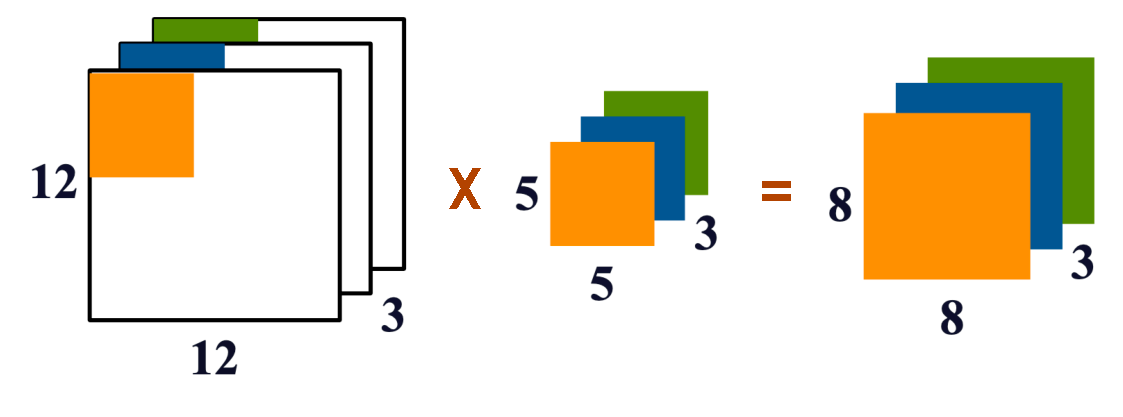
\includegraphics[height=2.5cm]{./figure/depthwisedemo.eps}
	\label{fig:dwdemo}}
\vspace{1em}
\subfloat[Pointwise convolution: four 3-channel $1 \times 1$ filters are used to convolve with one 3-channel $8 \times 8$ input and generate one 4-channel $8 \times 8$ output.]{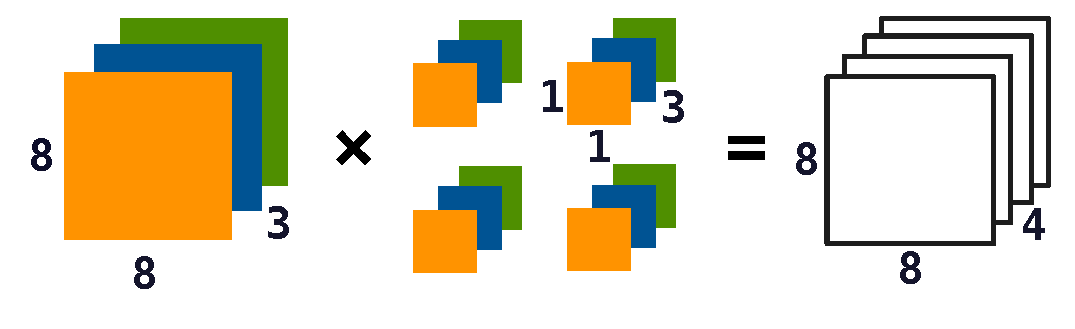
\includegraphics[height=2.5cm]{./figure/pointwisedemo.eps}
	\label{fig:pwdemo}}
\caption{Demonstration of depthwise and pointwise convolutions.}
  \label{fig:depsepconv}
\end{figure}

\subsection{Depthwise Separable Convolution}
Our work targets depthwise separable convolution (DSC) that is widely used by  CNN  models to reduce the number of multiplication
operations needed for doing convolution (a standard operation in CNN). The DSC splits a standard (e.g., multi-channeled) 2D
convolution kernel into two individual kernels: a depthwise convolution kernel and a pointwise convolution kernel. 

The depthwise
convolution kernel processes one input channel at a time, and stacks the outputs of all channels together to form an $n \times n \times c$
matrix, where $n \times n$ is the output of a depthwise convolution kernel and $c$ is the number of channels to be processed. Specifically,
it takes as input a feature map and applies a bank of 2D filters (e.g., an $N \times N$ kernel) on the width and height directions of
the input. We iteratively apply the depthwise convolution kernel to all channels. Fig. \ref{fig:dwdemo} shows an example of depthwise convolution, where three $5 \times 5$ 2D filters are used to convolve with the corresponding channel of a $12 \times 12 \times 3$ feature map and generate one $8 \times 8 \times 3$ output. 

The output of the depthwise convolution kernel is fed
into a pointwise convolution kernel which uses a $1 \times 1$ filter to iterates through every single point. This kernel has a depth of the
number of input channels (i.e., $c$). The DSC reduces the computation by reducing the number of input transformations needed when compared
to a standard depthwise convolution. Fig. \ref{fig:pwdemo} shows an example of pointwise convolution, where four $1 \times 1 \times 3$ filters are used to convolve with the $8 \times 8 \times 3$ feature map iteratively and each filter generate one channel of a $8 \times 8 \times 3$ output.


\subsection{Roadmap and Notations} We present our approach for optimizing the two convolutional kernels of DSC in
Sections \ref {sec:strategies} and \ref {sec:pwconv}. We start by introducing our methods for improving data locality of depthwise
convolution in Section \ref{sec:strategies} and then presenting our approach for using dynamic work distribution to accelerate
small-batch-sized pointwise convolution in Section \ref {sec:pwconv}.

\mypara{Notations.} Throughout the paper, we use $I$, $F$, and $O$ to represent the input, the filter, and the output respectively; we also
use $N$, $C$, $H$, and $W$ to denote the batch size, the channel, the height, and the width, respectively.

\section{Our Approach}
\label{sec:strategies} In this section, we describe our two optimizations, column reuse (Section \ref{sec:creuse}) and row reuse (Section
\ref{sec:rowreuse}), for reducing GPU memory transactions for convolution operations. In Section \ref{sec:together}, we show how the two
optimizations can be used together.

%\subsection{Preliminaries}
%
%Our approach optimizes convolution operations on GPUs by reusing column and row elements. Throughout the paper, we use $I$, $F$, and $O$ to
%represent the input, the filter, and the output respectively, $N$, $C$, $H$, and $W$ to denote the batch size, the channel, the height, and
%the width, respectively.

\subsection{Column Reuse Optimization}
\label{sec:creuse}

\begin{figure*}[!t]
\centering
\subfloat[Direct convolution: Each thread loads 5 input elements from global memory.]{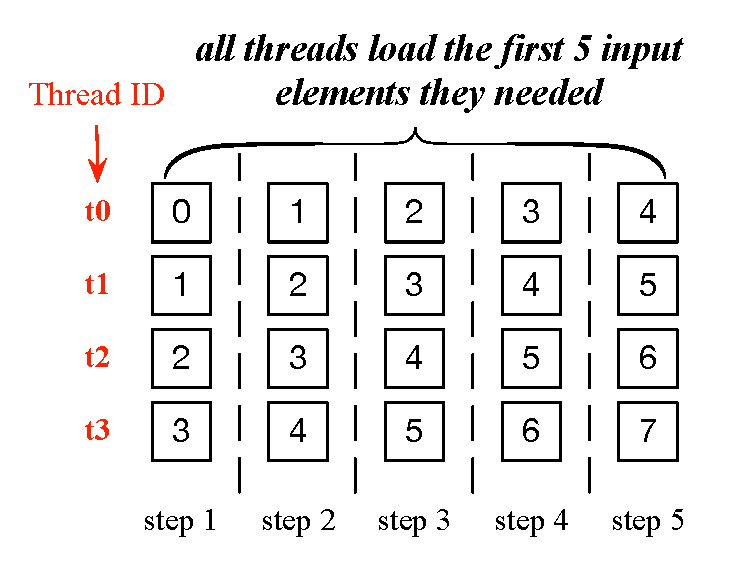
\includegraphics[width=0.3\textwidth,height=3.2cm]{./figure/directconv.eps}
	\label{fig:directalgo}}
\hspace{0em}
\subfloat[Optimized convolution: each thread retrieves its third element from the corresponding thread.]{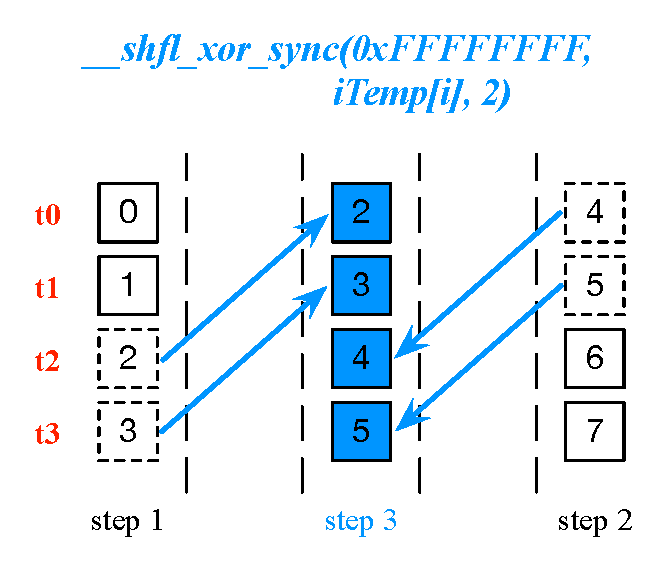
\includegraphics[width=0.3\textwidth,height=3.2cm]{./figure/optalgo1.eps}
	\label{fig:optalgo1}}
\hspace{0em}
\subfloat[Our approach: each thread retrieves its second and fourth elements from corresponding threads.]{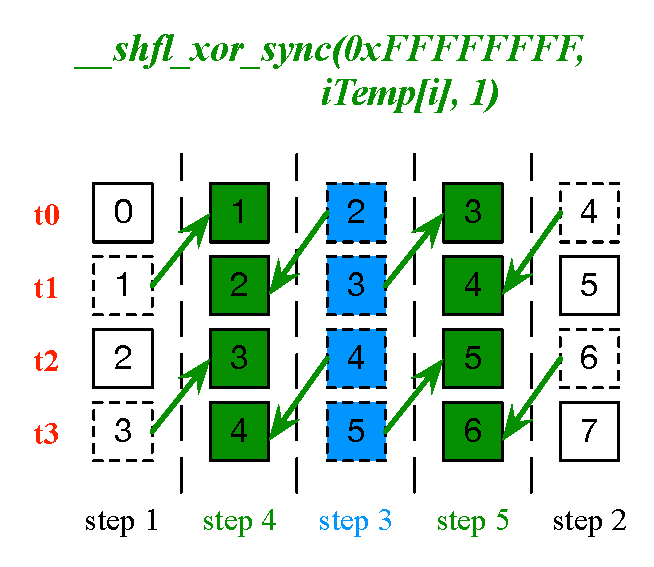
\includegraphics[width=0.3\textwidth,height=3.2cm]{./figure/optalgo2.eps}
	\label{fig:optalgo2}}

\caption{Illustration of direct and optimized convolution. We use a $5 \times 5$ filter  and each thread calculates the convolution for one
output element. This example shows how a thread processes the first 5 corresponding input elements.} \label{fig:corealgo}
\end{figure*}

\mypara{Working example.} We use the 2D convolution example shown in Figure \ref{fig:twostrategies} as a working example to explain our
column reuse method. Here, we slide a $5 \times 5$ filter over a $6 \times 11$ image to produce a $2 \times 7$ output. In this example,
each thread calculates one column of the output. Two parallel threads 0 and 1 will execute code to slide the filter along the width
dimension, where both threads load two overlapped regions from the input image (thereby generating four duplicate columns). Similarly,
there will be another thread (thread 6 in this example) to slide the filter along the height dimension, which will load two overlapped
regions and generates four duplicate rows.



\subsubsection{Standard convolution} Figure \ref{fig:directalgo} shows a standard 2D convolution operation, operating on one single channel
of the input (e.g., an image). Here, each thread loads the first corresponding input elements from the GPU global memory. Given that the
indices of these elements are contiguous, i.e., 0, 1, 2, and 3 in this example, concurrent access to these elements will be coalesced to
form a single memory transaction. As a result, each step will incur one memory transaction, five for the five steps (steps 1-5) as shown in
Figure \ref{fig:directalgo}. After completing step 5, each pair of adjacent threads will have four duplicate input elements, corresponding
to the duplicate columns in Figure \ref{fig:twostrategies}. Specifically, input elements 1, 2 and 3 loaded in step 2 would have already
been loaded by threads $t1$, $t2$ and $t3$ in the previous step (Figure \ref{fig:directalgo}). The repeated load to these elements lead to
redundant memory accesses and unnecessary memory access overhead. Even the elements may be prefetched to the L1 cache before the next step,
access to the L1 cache still takes around 30 cycles on a GPU. To reduce the memory overhead, we would like to avoid such redundant memory
accesses.


\subsubsection{An optimized version} To eliminate the redundant loads, we could use the shuffle instructions to exchange input elements among
different threads.   Figure \ref{fig:optalgo1} depicts such an optimization. Specifically, in steps 1 and 2 of Figure \ref{fig:optalgo1},
each thread loads the corresponding first and fifth input elements from the global memory. In step 3, each thread utilizes the shuffle
instruction to retrieve the third element from another thread. For example, threads $t0$ and $t1$ could retrieve the third element from
threads $t2$ and $t3$, respectively, and provide the fifth element (dashed squares in step 2) for both threads. Similarly, threads $t2$ and
$t3$ retrieve the third element from threads $t0$ and $t1$, respectively, and provide the first element (dashed squares in step 1) for
threads $t0$ and $t1$. Using the CUDA shuffle instruction, this exchange process can be implemented as $shfl\_xor(iTemp[i],2)$, where
$iTemp$ is a thread-local array used to store the five input elements, and $i$ is the location in the local array. In our case, threads
$t0$ and $t1$ will supply the fifth element, hence $i=4$. Similarly, threads $t2$ and $t3$ will provide the first element, thus $i=0$.



While this version reduces the redundant memory accesses compared to a standard convolution implementation, there is still room for
improvement. The problem is that the shuffle instruction $shfl\_xor(iTemp[i],2)$ now becomes a bottleneck because $iTemp$ is accessed
through dynamic indexing. Since the indices and the access pattern to $iTemp$ are not available at compile-time, the compiler cannot decide
which of the elements in $iTemp$ will be frequently accessed and has to place $iTemp$ in the local memory which would still incur an access
latency of around 500 cycles. If we can promote register allocation for $iTemp$, we can then further improve the performance of
convolution.


\subsubsection{Our approach}
Our column reuse approach (Figure \ref {fig:optalgo2}) converts dynamic indexing to static array access. This strategy promotes register
allocation, leading to better performance over the optimized version shown in Figure \ref{fig:optalgo1}.

Our approach is described in Algorithms \ref{algo:basic} and \ref{algo:basic2},
where the first algorithm is used for step 3, and the later is used for steps 4 and 5. Note that these two algorithms can be used for
different sized convolution kernels, for which we will discuss in Section \ref {sec:rowreuse}.

Figure \ref{fig:exchange} shows the process of Algorithm \ref{algo:basic}. Here, we first load the corresponding first and fifth input elements
into $iTemp$ before passing it to Algorithm \ref{algo:basic}. Then, we pack two 32-bit elements into a 64-bit variable $exchange$, where
$iTemp[4]$ and $iTemp[0]$ are the high and low 32 bits, respectively (Line 2).  As threads $t0$ and $t1$ will provide the fifth element of
the data they load, which are the high 32 bits of $exchange$, we right shift $exchange$ for both threads by an offset of 32 to place
$iTemp[4]$ in the low 32 bits. Turning our attention to threads $t2$ and $t3$ that will provide the first element of the data they loaded.
Since the elements are already the low 32 bits of $exchange$, we right shift $exchange$ in both threads by an offset of 0. The number of
places to be shifted for each thread is calculated based on the thread ID (Line 3). Next, we unpack $exchange$ into $iTemp[2]$ (high 32
bits) and $iTemp[1]$ (low 32 bits) (Line 5). By doing so, we can retrieve the element a thread needs to supply from a fixed location,
$iTemp[1]$. Finally, we use the shuffle instruction to exchange the elements among the threads (Line 6).


\begin{algorithm}[t!]
\small

\tcp{$iTemp$: Buffer for storing input elements loaded from memory or generated through  \emph{shuffle} instructions.}
%\tcp{$iTemp$ contains input elements either loaded from global memory or through \emph{shuffle} instructions.}
\KwIn{$iTemp$}
	\KwOut{$iTemp$}
	$tid \gets threadIdx.x$\;
	$mov\ exchange, \{iTemp[0], iTemp[4]\}$\;
	$shift \gets ((tid+2)\&2)<<4$\;
	$exchange \gets exchange >> shift$\;
	$mov\ \{iTemp[1],iTemp[2]\}, exchange$\;
	$iTemp[2] \gets shfl\_xor(iTemp[1],2)$\;	
	
	\caption{RetrieveThirdElement}
	\label{algo:basic}
	
\end{algorithm}

Using Algorithm \ref{algo:basic}, we can replace the compile-time undecidable dynamic index $i$ in $shfl\_xor(iTemp[i],2)$ with static
indexing $1$ in $shfl\_xor(iTemp[1],2)$ of our working example. By doing so, we promote register allocation by allowing the compiler to put
all the thread-local variables into the fast GPU registers (that have access latency of 1 to 2 cycles as opposed to 500 cycles when the
data are stored in the local memory). Since steps 4 and 5 of our implementation (Figure \ref{fig:optalgo2}) adopt a similar procedure as
step 3 in Figure \ref{fig:optalgo1}, we can adapt Algorithm \ref{algo:basic} to obtain Algorithm \ref{algo:basic2} with minor
modifications. The main distinction between the two algorithms comes from how we process steps 3-5 shown in Figure \ref{fig:optalgo2}.
Specifically, we use four threads to exchange the elements in step 3 for Algorithm \ref{algo:basic}, but use only two adjacent threads in
step 4 and 5 for Algorithm \ref{algo:basic2}. To adapt to the change of the number of threads used, we recalculate the shift offset for
each thread (Line 3 of both algorithms) and change the arguments of the shuffle instruction (Line 6 in both algorithms).


For this working example, Algorithms \ref{algo:basic} and \ref{algo:basic2} respectively reduce the number of memory transactions from 5 to
2 and 25 to 10 when 5 and 25 input elements are loaded. This reduction greatly improves the performance of the convolution.

\subsubsection{Generalization} While we have described our approach using a concrete working example with a pre-defined filter size, our
algorithms can be generalized to filters with an arbitrary size. To apply our approach to a filter of size $n \times n$, we will first
divide the filter into a number of $n \times 5$ sub-filters. Next, we divide remaining columns into a number of $n \times 3$ sub-filters
with some overlap columns. For example, a $7 \times 7$ filter can be divided into a $7 \times 5$ sub-filter and a $7 \times 3$ sub-filter
with one overlap column. Each $n \times 5$ and $n \times 3$ filters can be processed by Algorithm \ref{algo:basic} and Algorithm
\ref{algo:basic2}.






\begin{figure}[t!]
	\centering
	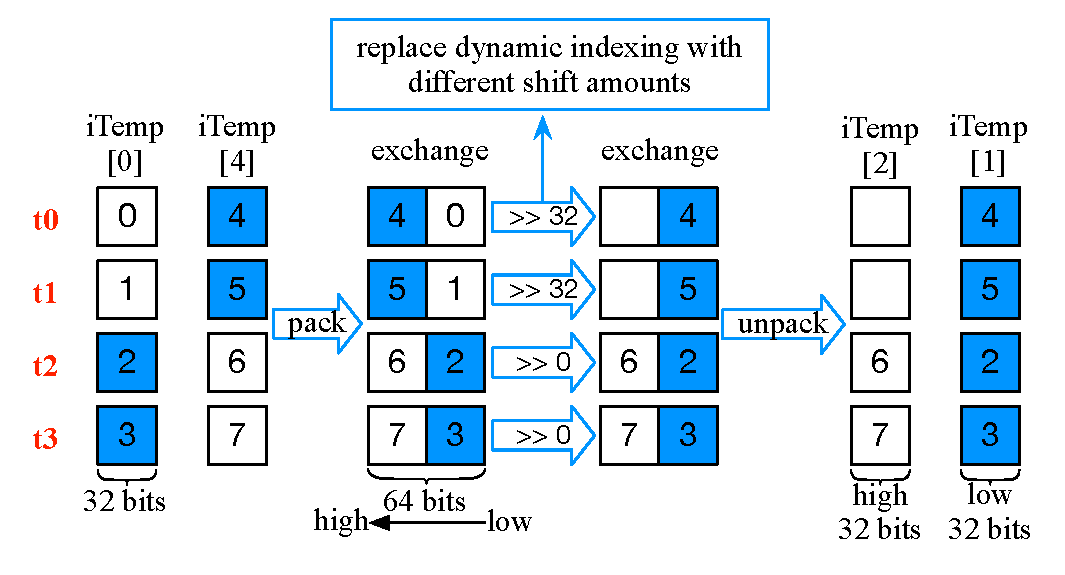
\includegraphics[width=0.8\columnwidth,height=3.5cm]{./figure/exchange.eps}
\caption{Convert the dynamic indexing of array $iTemp$ into static indexing. This allows the compiler to allocate $iTemp$ in registers instead of local memory.}
\label{fig:exchange}
\end{figure}


\begin{algorithm}[t!]
\small
	\KwIn{$iTemp$}
	\KwOut{$iTemp$}
	$tid \gets threadIdx.x$\;
	$mov\ exchange, \{iTemp[0], iTemp[2]\}$\;
	$shift \gets ((tid+1)\&1)<<5$\;
	$exchange \gets exchange >> shift$\;
	$mov\ \{iTemp[0],iTemp[1]\}, exchange$\;
	$iTemp[1] \gets shfl\_xor(iTemp[0],1)$\;	
	\caption{RetrieveSecondElement}
	\label{algo:basic2}
\end{algorithm}


\subsection{Row Reuse Optimization}
\label{sec:rowreuse}
\begin{figure}
	\centering
	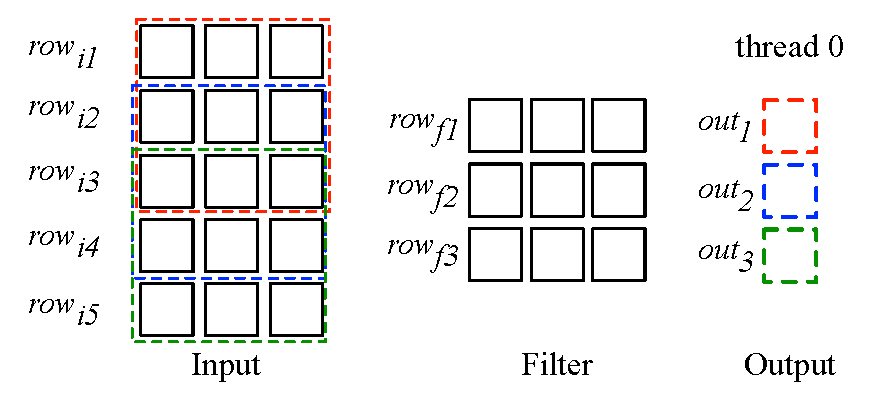
\includegraphics[width=0.8\columnwidth,height=3cm]{./figure/rowreuse.eps}
\caption{A $3 \times 3$ filter is used to slide over the input image along height dimension, which produces a column of output elements.}
\label{fig:rowreuse}
\end{figure}

\mypara{Working example.} Consider the standard convolution example shown in Figure \ref{fig:rowreuse} as a working example for row reuse
algorithm. When sliding the filter over the input image along the height dimension, it produces a column of elements as the output.


\subsubsection{Standard convolution} Assume we use use one thread to calculate one column of output elements. For the working example given in Figure
\ref{fig:rowreuse}, the convolution will be computed as follows:

\begin{gather*}
  out_0=row_{i0} \cdot row_{f0} + row_{i1} \cdot row_{f1} + row_{i2} \cdot row_{f2} \\
out_{1}=row_{i1} \cdot row_{f0} + row_{i2} \cdot row_{f1} + row_{i3} \cdot row_{f2} \\
out_{2}=row_{i2} \cdot row_{f0} + row_{i3} \cdot row_{f1} + row_{i4} \cdot row_{f2}
\end{gather*}

The above equations suggest that $row_{i1}$ and $row_{i3}$ are loaded twice, and $row_{i2}$ is loaded three times; nine rows should be
loaded in total. The redundant loads to the same read-only row thus incur extra memory transactions and additional overhead.



\subsubsection{Our optimization}
To remove redundant loads to the same row, we redesign the execution flow of the convolution. Specifically, after loading a row from the
input, we compute the number of output elements that depend on the loaded row. For our working example, the computation of element $out_0$
in the output column would depend on $row_{i0}$. Similarly, output elements $out_0$ and $out_1$ will need $row_{i1}$. With this information
in place, we use the loaded row to perform inner product with corresponding rows of the filter to calculate the output elements whose
outcomes depending on the loaded row. Our approach translates the execution flow of the working example presented in Figure \ref
{fig:rowreuse} to:

\begin{equation}\nonumber
\begin{aligned}
load\ row_{i0}:
&\ out_0=row_{i0} \cdot row_{f0} \\
load\ row_{i1}:
&\ out_0 = out_0+row_{i1} \cdot row_{f1}\\
&\ out_1=row_{i1} \cdot row_{f0}\\
load\ row_{i2}:
&\ out_0 = out_0+row_{i2} \cdot row_{f2}\\
&\ out_1 = out_1+row_{i2} \cdot row_{f1}\\
&\ out_{2}=row_{i2} \cdot row_{f0}\\
load\ row_{i3}:
&\ out_1=out_1+row_{i3} \cdot row_{f2} \\
&\ out_2=out_2+row_{i3} \cdot row_{f1}\\
load\ row_{i4}:
&\ out_2=out_2+row_{i4} \cdot row_{f2}
\end{aligned}	
\end{equation}



In this new implementation, we would only issue loads to five rows to calculate the output elements. Compared to the nine loads required by
the standard convolution implementation, we reduce the number of loads to row elements by nearly half.  We note that although the number of
accesses to the output column $out$ is increased, the overhead is negligible because $out$ is much smaller than multiple rows and hence can
be stored in registers.

We describe a general solution for row reuse in Algorithm \ref{algo:rowreuse}, where $row$ denotes the row loaded from the input, $index$
denotes the index of $row$, $filter$ denotes the vector of filter rows and $filter[i]$ means the $i$th row of the filter. Pesudo code at
Lines 1-5 process the first $F_H-1$ rows ($row_{i0}$ and $row_{i1}$ in Figure \ref{algo:rowreuse}) that are needed by less
than $F_H$ output elements. Code at lines 6-11 process the rows that are needed by exact $F_H$ output elements (e.g., $row_{i2}$ in Figure
\ref{algo:rowreuse}). Finally, code at Lines 12-17 process the last $F_H-1$ rows, which are needed by less than $F_H$ output elements
(e.g., $row_{i3}$ and $row_{i4}$ in Figure \ref{algo:rowreuse}).


\begin{algorithm}[t!]
\small
	\KwIn{$row$, $index$, $filter$, $Out$}
	\KwOut{$Out$}
	\If{$index \textless F_H-1$}{
		\For {$i \gets 0$ \KwTo $index+1$}{
			$Out[i] \gets Out[i]+row \cdot filter[index-i]$\;
		}
	}\ElseIf{$index \geq F_H-1$ \textbf{and} $index \textless I_H-F_H+1$}{
		\For {$i \gets 0$ \KwTo $F_H$}{
			$o_{index} \gets index-F_H+1+i$\;
			$Out[o_{index}] \gets Out[o_{index}]+row \cdot filter[F_H-1-i]$\;
		}
	}\Else{
		\For {$i \gets F_H-1$ \KwTo $0$}{
			$o_{index} \gets I_H-F_H+1$\;
			$Out[o_{index}] \gets Out[o_{index}]+row \cdot filter[F_H-i]$\;
		}
	}
	\caption{Row Reuse Algorithm}
	\label{algo:rowreuse}
\end{algorithm}

Algorithm \ref{algo:rowreuse} is designed to eliminate redundant loads to the same row introduced by sliding a filter over the input along
the height dimension. By loading each row of the input just once, our approach greatly reduces the number of memory transactions for
convolution operations.

\subsection{Putting Together}
\label{sec:together}
\begin{figure}
	\centering
	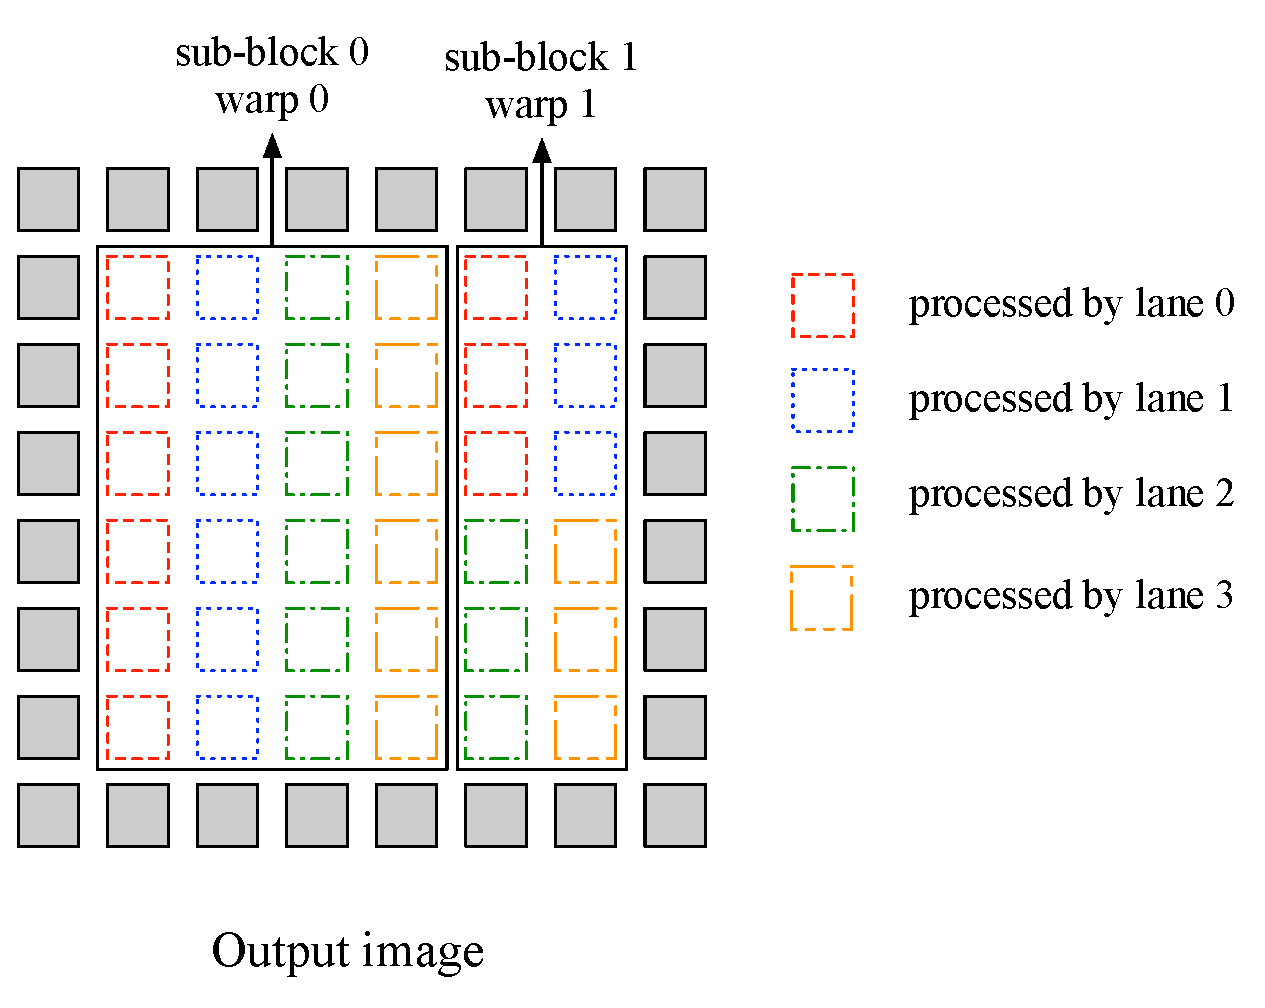
\includegraphics[width=0.8\columnwidth,height=5cm]{./figure/overalldesign.eps} 
	\vspace{-3mm}
	\caption{The output is produced by sliding a $3 \times
3$ filter over an $8 \times 8$ input with one pad. Here, we assume
that the warp size is 4 and thus having $laneid=threadid\%4$.} \label{fig:overalldesign}
\end{figure}


We have individually demonstrated how our column and row reuse optimizations can be used together to optimize GPU memory accesses for
depthwise convolution operations. We now take the widely used 2D convolution as an example to illustrate how to apply both reuse algorithms
on convolution operations.


To apply our approach to depthwise convolution that works on a 2D matrix, we first divide the output into sub-blocks. Each sub-block
contains exactly $n$ columns (in this work, $n = 32$, which is the default warp size of our GPU platform). The only exception is the last
sub-block, which may contain less than $n$ columns. If a sub-block contains more than $k$ rows ($k=56$ in this work), we then further
break down the sub-block along the height dimension. Each GPU thread block will process one or multiple sub-blocks, and each warp will
compute one sub-block. As a result, the threads within the same warp will process the adjacent columns of one sub-block.


\begin{algorithm}[t!]
\small
	\KwIn{$I$, $F$, $subBlockHeight$}
	\KwOut{$O$}
	Load the filter into shared memory\;
	Divide columns of the filter into a combination of 3-column and 5-column sub-filters\;
	$\_\_syncthreads()$\;
	\If{$blockIdx.x \textless gridDim.x-1$}{
		Init thread local register array $sum$ to zero\;
		Calculate the index of the first input element this thread needs, denoted as $inputIndex$\;
		\For{$i \gets 0$ \KwTo $subBlockHeight$}{
			\ForEach{sub-filter}{
				Load corresponding input elements from $inputIndex$ of global memory into $iTemp$\;
				Call $RetrieveThirdElement(iTemp)$ or $RetrieveSecondElement(iTemp)$\;
				Call $RowReuse(iTemp,i,$\textit{sub-filter}$,sum)$\;
			}
			Write completed element of $sum$ into $O$\;
		}		
		
	}
	\Else{
		Divide columns of the last sub-block into multiple partitions and try to evenly assign those partitions to threads of a warp. Each thread uses a direct method to calculate elements of $O$.\;
		The same method is adopted when processing the edge elements of $O$\;
	}
	\caption{Depthwise Convolution}
	\label{algo:overalldesign}
\end{algorithm}

\subsubsection{Example} Fig. \ref{fig:overalldesign} shows the mapping process of GPU threads to output elements. In this example, we slide a $3
\times 3$ filter over an $8 \times 8$ input. To apply a square  filter at the edge of the image, we need to pad the input. To reduce the
memory pressure, we do not allocate GPU memory space for the padded elements. Instead, we use different methods to calculate the edge and
inner elements of the output. The edge and inner elements are represented by the shaded and dashed squares in Fig.
\ref{fig:overalldesign}, respectively.


In this example, we assume each GPU warp contains four threads. Therefore, we will divide the inner elements into multiple sub-blocks and
each sub-block contains four columns so that a column can be processed by one of the four GPU threads within a wrap. In our case, we will
have two sub-blocks, where sub-block 0 contains four columns, but sub-block 1 only contains two columns. To utilize the threads within a
warp, we divide elements of the last two columns evenly among the four threads.

\subsubsection{Generalization} In Algorithm \ref{algo:overalldesign}, we describe our generalized solution. Here, we process the sub-blocks
with exactly 32 columns (i.e., the default wrap size of our evaluation GPU) and the last sub-block in Lines 4-15 and 16-19, respectively.
In this way, each GPU thread calculates one column of the output elements. This is done through several steps. First, each thread block
loads the filter into shared memory and divides the filter into a combination of 3-column and 5-column sub-filters. Next, each thread
calculates the address of the first input element it needs (Lines 6). For each output element and sub-filter, each thread loads
corresponding input elements into $iTemp$ and passes $iTemp$ to Algorithms \ref{algo:basic} and \ref{algo:basic2} to fill the row vector $iTemp$
(Line 10). Then, each thread passes the filled vector $iTemp$ to Algorithm \ref{algo:rowreuse} to calculate multiple output elements and
store results in the register array $sum$ (Line 11). Finally, when the calculation of one output element is completed, we write the
corresponding result in $sum$ into the result array $O$ (Line 13).

\section{Optimizing Pointwise Convolution}
\label{sec:pwconv} In this section, we explain the workflow of our dynamic block size scheme for pointwise convolution. This process is
depicted Fig. \ref{fig:pwworkflow} and consists of two stages, described as follows.

In the first stage, we use a 2-level hierarchical partitioning method to decompose the output into two levels of tiles, including block
tiles and warp tiles. Each thread block processes one block tile and each warp processes one warp tile. The main consideration when
decomposing the output is the layout of tiles on each level. In the second stage, we distribute channels of input or filter across threads
within a GPU warp. To achieve the best performance, we need to determine the number of channels to be distributed, the height of a warp
tile, and the number of thread blocks per SM (see also Section \ref{sec:ga}).

\subsection{2-Level Hierarchical Partitioning}
Our hierarchical partitioning method is governed by two parameters, the number of warps in a thread block, denoted as $Warp_{num}$, and the
number of thread blocks that can run concurrently on an SM, denoted as $Block_{num}$. We need to find the right warp number because a small
warp number will decrease the opportunity to hide the memory access latency at the warp level, but a large warp number will decrease the
number of thread blocks and may lead to SM underutilization. We empirically set the warp number to be four, which gives good performance on
our pilot study using microbenchmarks of hand-written depthwise convolution kernels. For the number of thread blocks, $Block_{num}$, we use
two values, 2 and 4, on our evaluation platforms. These choices are justified as follows. For Nvidia GPUs, each GPU thread can use up to
255 registers, and each SM has 65,536 registers. If we set $Block_{num}=1$ and $Warp_{num}=4$ (per our discussion above), each SM will have $Block_{num} \times Warp_{num}=4$ wraps. This allows a thread block to use up to just half of the available registers of an
SM because a thread block under this setting can use at most $4\ (warps\ in\ an SM) \times 32\ (threads\ per\ warp) \times 255\ (registers\ per\ thread)=32,640$ registers. Therefore, to utilize the available hardware register, one should set $Block_{num}$ to be greater than one. We
also found that using more than 4 threads per block offer little benefit and hence we set the $Block_{num}$ to be either 2 or 4 (to keep
this parameter a power of two value).

The workflow of our 2-level hierarchical partitioning method is illustrated in Fig. \ref{fig:pwworkflow}. First, we describe how to
partition a block tile into warp tiles, and second, how to partition the output into block tiles.

We halve both dimensions of each block tile and generate $2 \times 2$ warp tiles. The height and width of a warp tile are represented as
$Warp_H$ and $Warp_W$ respectively. In our design, when $Warp_H > 12$, we need assembly level optimizations like the work in
\cite{yan2020optimizing,yan2020demystifying} for some configurations of pointwise convolution to avoid register spills. But in this work,
we focus on higher level rather than assembly level optimizations, and thus set $Warp_H \leq 12$.

To divide the output into block tiles, we use two logical layouts of the output, \textbf{\emph{L1}} and \textbf{\emph{L2}}, as shown in Fig. \ref{fig:pwworkflow}.
$F_N$ and $I_N \times I_H \times I_W$ represent the filter and input dimensions of the output respectively.
Before partitioning the output, we first select the layout of the output based on the size of the filter dimension.
The rationale behind this choice can be described as follows.
The number of filters, $F_N$, is fixed once the structure of a CNN is determined.
But the size of the input dimension will be affected by the batch size, $I_N$, during inference and training.
Therefore, it is easier to distribute channels of filters than inputs in our approach.
For the sake of simplicity, we design our partition method to utilize layout \textbf{\emph{L1}} whenever there are enough filters to be distributed across threads.
Specifically, when $F_N \ge 48$, we choose layout \textbf{\emph{L1}} and distribute filter channels across threads within a warp.
Otherwise, we choose layout \textbf{\emph{L2}} and distribute input channels.
The boundary $F_N = 48$ is determined as follows.
Fig. \ref{fig:pwworkflow} demonstrates that in layout \textbf{\emph{L2}}, the maximal value of $F_N$ is $4 \times Warp_H$ and $Warp_H \leq 12$, therefore we have $F_N \leq 48$ in layout \textbf{\emph{L2}}.

After choosing the layout, we partition the output along the filter dimension.
For the layout \textbf{\emph{L1}}, we halve the filter dimension if $F_N \geq 512$.
The reason is that if we let each thread block process a large number of filters, then each thread needs to issue more load instructions, which may cause MIO (Memory Input Output) instruction queue throttle and leads to performance degradation.
For the layout \textbf{\emph{L2}}, we halve the filter dimension if $F_N \geq 24$.

\subsection{Distribute Channels Across Threads}
In this stage, we distribute channels of filters or inputs across threads within a warp.
The number of channels to be distributed is denoted as $C_{num}$.
To achieve the best performance, we iterate over all candidate combinations of $Block_{num}$, $C_{num}$ and $Warp_H$, and select the combination that leads to optimal SM utilization and arithmetic intensity.

Now we illustrate how to determine candidates for $C_{num}$ and $Warp_H$ with layout \textbf{\emph{L1}}.
Layout \textbf{\emph{L2}} has a similar process.
Assume that we distribute 8 channels ($C_{num}=8$), meaning that 8 threads will load 8 channels of the same filter into registers.
Therefore, 32 threads of a warp can load 32 channels of $32/8=4$ filters at the same time, we denote this number as $F_{num}=32/C_{num}$.
And then the number of filters each thread needs to process can be calculated with $T_{num}=Warp_W/F_{num}$.
To fully utilize a warp, $C_{num}$ should be a power of 2.
Thus, candidates for $C_{num}$ are $C_{num}=\{1,2,4,8,16,32\}$.

Next, we demonstrate how to determine the candidates for $Warp_H$ based on the size of the input dimension, $I_N \times I_H \times I_W$.
If the size of the input dimension is large, we prefer to choose a large $Warp_H$ because using small $Warp_H$ will generate more thread blocks and results in multiple loads of shared filters \cite{jia2020enabling, zheng2020flextensor}.
If the size of the input dimension is small, we prefer to choose small $Warp_H$ because using a large $Warp_H$ will generate a few thread blocks and result in SM underutilization.
Since each thread loads at most 12 input elements ($Warp_H<12$), we set the upper limit of large $Warp_H$ to 12 and the lower limit to $12/2=6$.
Therefore, the candidates for large $Warp_H$ are $Warp_H=\{6,7,8,9,10,11,12\}$.
The candidates for small $Warp_H$ are $Warp_H=\{2,3,4,5,6,7,8\}$.
In our experiments, there is no clear boundary between large and small candidate sets of $Warp_H$, therefore we let both sets overlap in the middle values.
The boundary between the large and small size of the input dimension is experimentally determined as $I_N \times I_H \times I_W=16 \times 14 \times 14$.

When searching for the optimal combinations, we only consider combinations that satisfy hardware resources constraints, including registers and shared memory.
Based on $Block_{num}$, we calculate the number of registers each thread can use ($Limit_R$) and the size of shared memory each thread block can use ($Limit_S$) with formulas $Limit_R=Total_R/(Block_{num}\times Warp_{num} \times 32)$ and $Limit_S=Total_S/Block_{num}$ respectively. $Total_R$ and $Total_S$ represent the number of registers and the size of shared memory of an SM, respectively. On RTX 2080Ti, $Total_R=65536$ and $Total_S=64KB$ while  on Jetson AGX Xavier, $Total_R=65536$ and $Total_S=48KB$.
Each thread calculates $Warp_H \times T_{num}$ output elements and thus needs $R_O=Warp_H \times T_{num}$, $R_I=Warp_H$ and $R_F=T_{num}$ registers to store output elements, input elements and filter elements respectively.
In cases where the computational workload is small, we try to let each thread accumulates $Warp_H \times T_{num}$ output elements $k \in \{1,2,3,4\}$ times.
The constraints can be formulated as follows:
\begin{equation}\nonumber
R_{LF}=\frac{C_{num} \times k \times Block_W}{128},R_{LI}=\frac{C_{num} \times k \times Block_H}{128}
\end{equation}
\begin{equation}
    \label{fo:limitr}
R_O+R_I+R_F+R_{LF}+R_{LI}+extraR \leq Limit_R
\end{equation}
\begin{equation}
    \label{fo:limits}
(Block_H+Block_W)\times C_{num} \times k \times 4 \times 2 \leq Limit_S
\end{equation}
where $R_{LF}$ and $R_{LI}$ are the number of temporary registers used to store filter and input elements loaded from global memory respectively, $extraR$ is the number of additional registers allocated by the compiler. Values of $k$ and $extraR$ for each kernel are determined through an off-line method. In Formula \ref{fo:limits}, 4 means each element has 4 bytes and 2 means we use a double buffer method.
\begin{figure*}
	\centering
    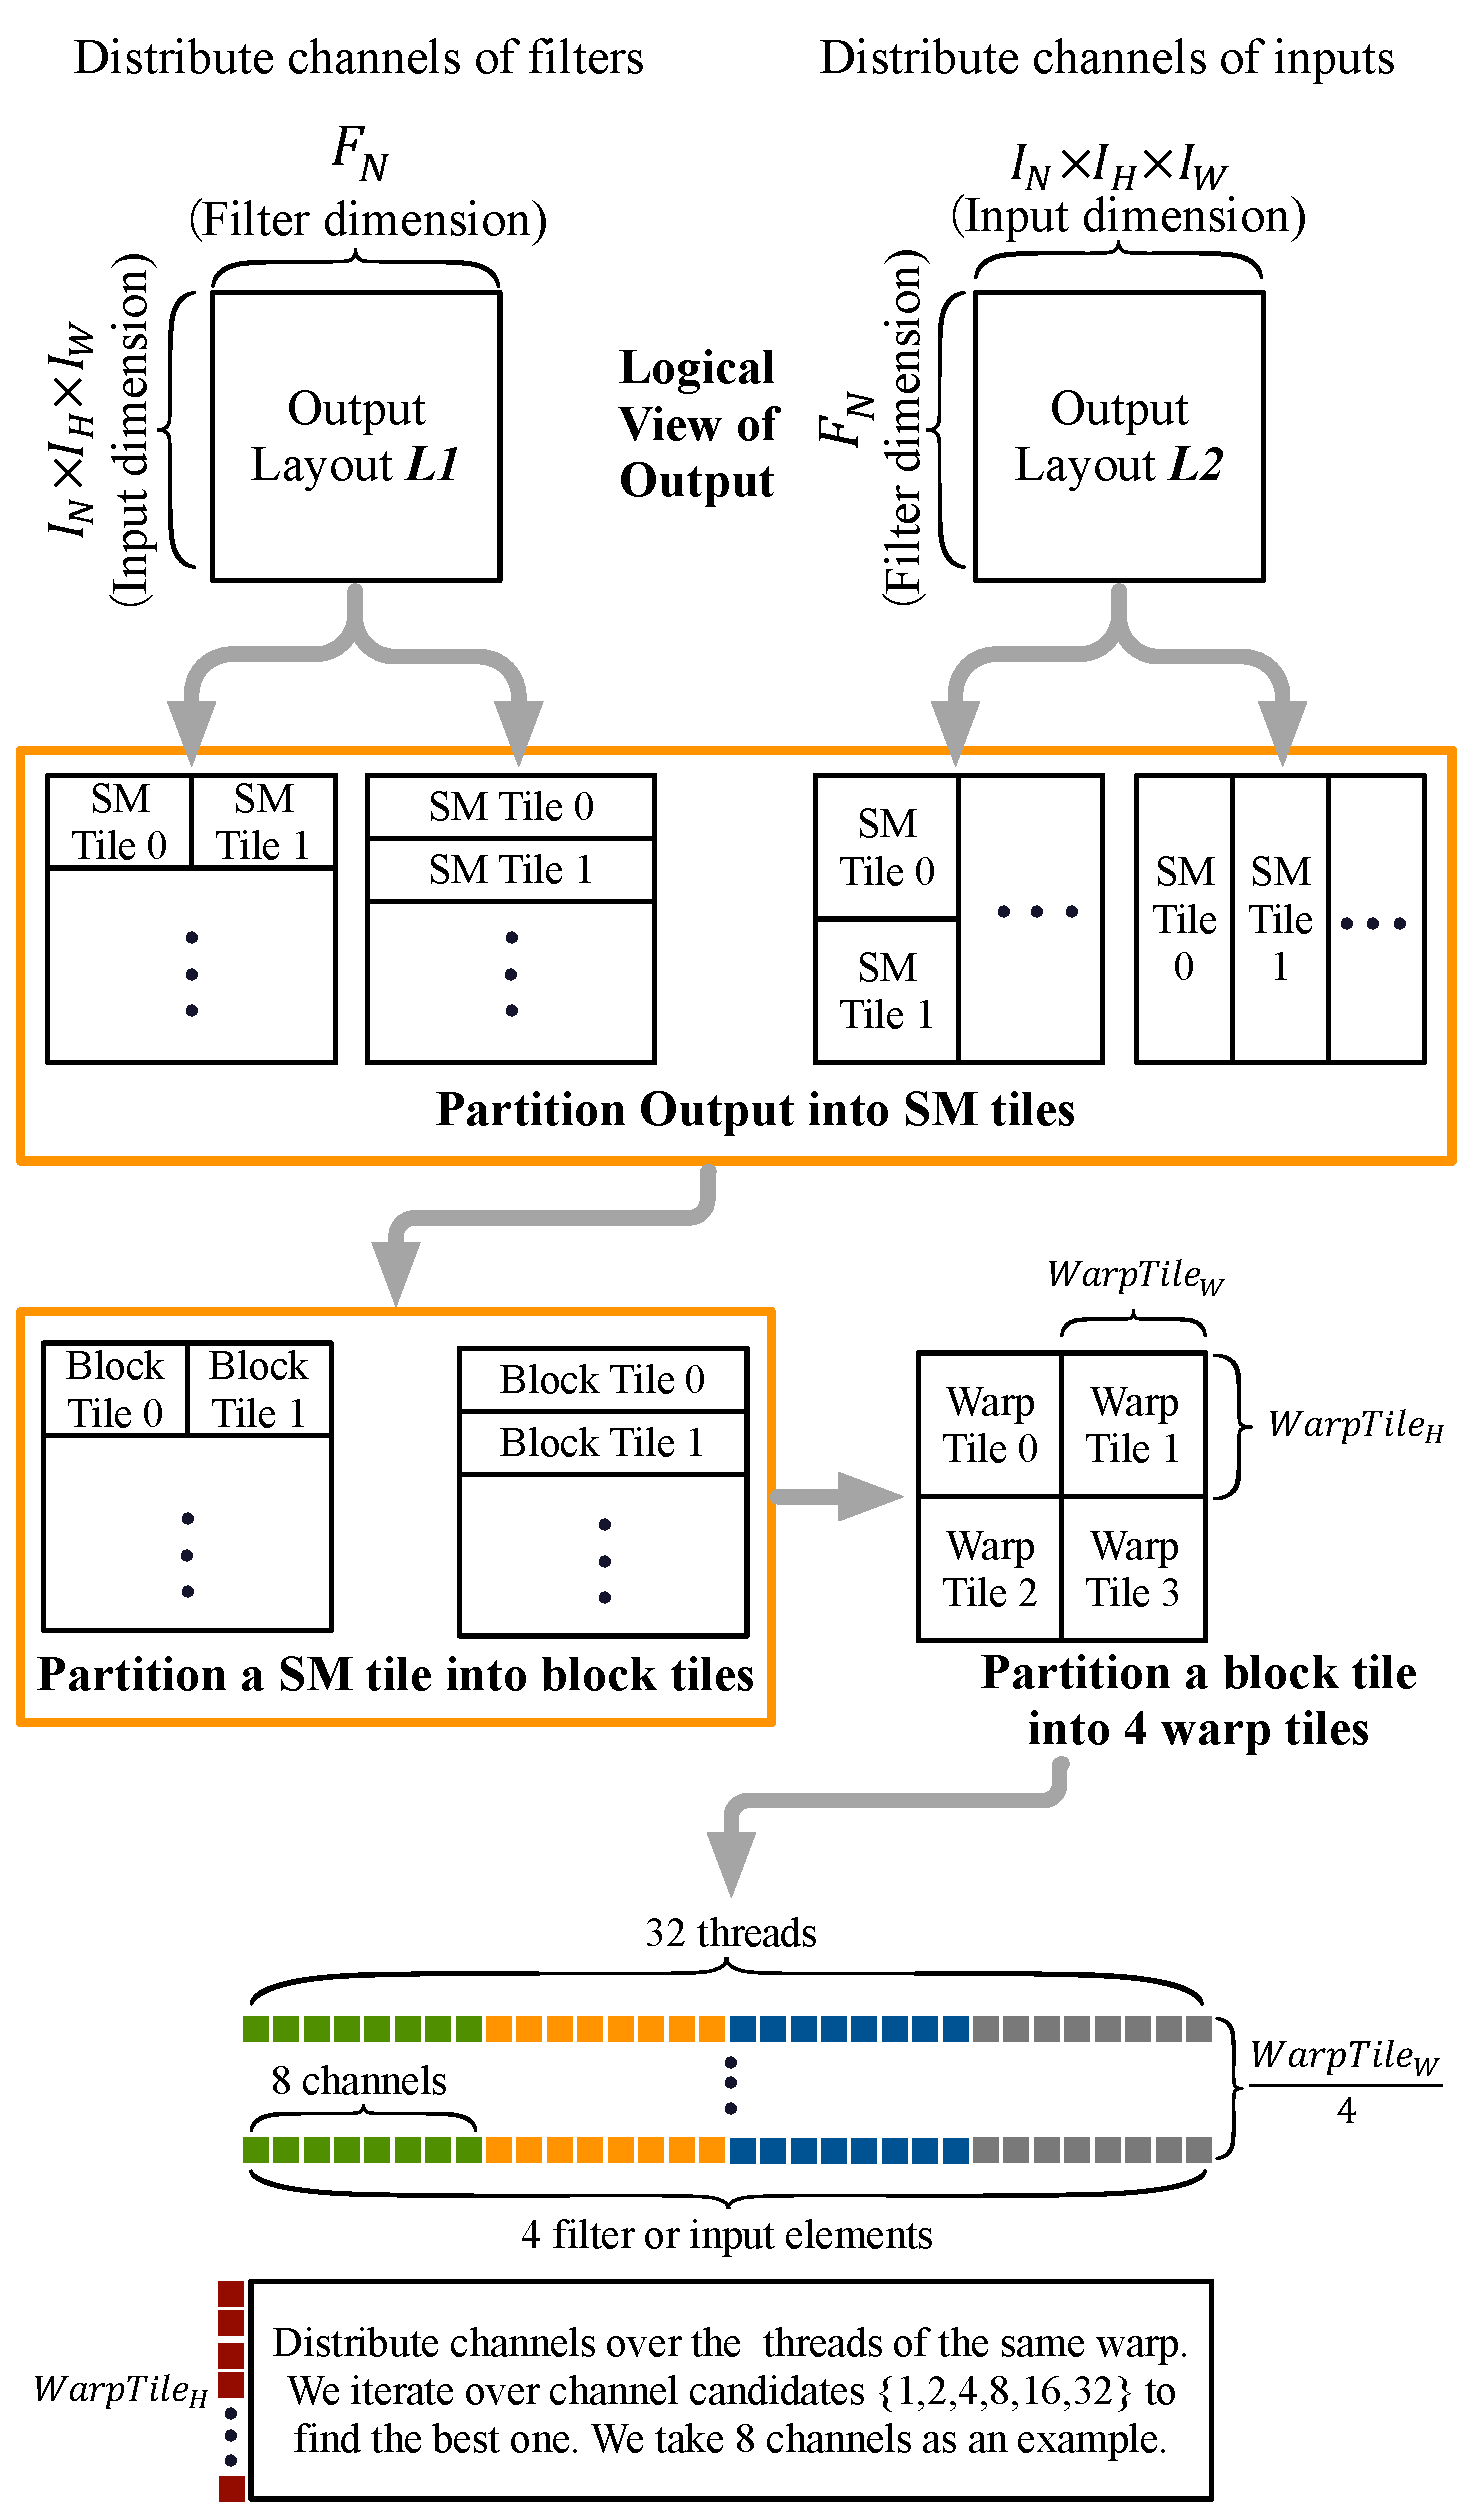
\includegraphics[width=0.95\textwidth,height=7cm]{./figure/pwworkflow.eps}
    \caption{Workflow of our dynamic block size method.} \label{fig:pwworkflow}
\end{figure*}
\begin{algorithm}[t!]
    \small
        \KwIn{$I$, $F$}
        \KwOut{$O$}
        \tcp{below codes are executed on CPU}        
        $Warp_{num} \gets 4$, $Block_{num} \gets \{2,4\}$\;
        $C_{num} \gets \{1,2,4,8,16,32\}$\;
        
        Choose the layout and partition the output based on $F_N$\;
        Choose the candidate set for $Warp_H$ ($Warp_W$) based on the size of input dimension\;
        $preSM \gets MAX\_FLOAT$,$preD \gets MAX\_INT$\;
        \ForEach{combination of $Block_{num}$, $C_{num}$ and $Warp_H$ ($Warp_W$)}{
            \If{not satisfy constraints of Formula \ref{fo:limitr} and \ref{fo:limits}}{
                continue\;
            }
            Calculate $SM_{util}$ and $D$ with Formula \ref{fo:smutil} and \ref{fo:diff}\;
            \If{$preSM \geq 1$ and $SM_{util} \geq 1$ and ((both are close and $D<preD$) or ($SM_{util}<preSM$))}{
                    $preSM \gets min(preSM,SM_{util})$\;
                    $preD \gets D$, record the combination\;
            }
            \ElseIf{$SM_{util}<1$ and ((both are close and $D<preD$) or ($SM_{util}>preSM$))}{
                    $preSM \gets max(preSM,SM_{util})$\;
                    $preD \gets D$, record the combination\;
            }

        }
        
        Choose the proper kernel based on the recorded $Block_{num}$, $C_{num}$ and $Warp_H$.\;
        \tcp{below codes are executed on GPU}
        Each thread block loads $k\times C_{num}$ channels of the needed input and filter into shared memory array $sharedBuf1$\;
        $\_\_syncthreads()$\;
        \For{$iter \gets 0$ \KwTo $I_C$ By $2 \times k \times C_{num}$}{
            Load next $k \times C_{num}$ channels of input and filter into temporary registers\;
            Load current channels of input and filter from $sharedBuf1$ into registers\;
            Accumulate output elements $k$ times\;
            Write temporary registers into shared memory $sharedBuf2$\;
            $\_\_syncthreads()$\;
            Repeat above steps but swap $sharedBuf1$ and $sharedBuf2$\;
        }
        Use segmented parallel reduce to get the final output elements and write the result to $O$\;
        \caption{Pointwise Convolution Optimization}
        \label{algo:pwalgo}
\end{algorithm}

To guide the search for the optimal combination of $Block_{num}$, $C_{num}$ and $Warp_H$, we use two metrics named SM utilization ($SM_{util}$) and the difference between $Warp_H$ and $T_{num}$ ($D$).
Two metrics can be calculated as follows:
\begin{equation}\nonumber
    Block_{count}=\frac{F_N}{Block_W} \times \frac{I_N \times I_H \times I_W}{2 \times Warp_H}
\end{equation}
\begin{equation}
    SM_{util}=\frac{Block_{count}}{Block_{num}\times SM_{num}}
    \label{fo:smutil}
\end{equation}
\begin{equation}
    D = |Warp_H-T_{num}|
    \label{fo:diff}
\end{equation}
where $Block_{count}$ is the number of generated thread blocks, $SM_{num}$ is the number of SMs on a GPU. For RTX 2080Ti and AGX Xavier, $SM_{num}=68$ and $SM_{num}=8$ respectively.

We will demonstrate how to select the optimal combination based on both metrics in the next section.

\subsection{Putting Together}
The whole workflow is described in Algorithm \ref{algo:pwalgo}.
We first choose the layout of output and partition the output into block tiles based on $F_N$ (Line 3).
Second, we choose the candidate set for $Warp_H$ based on $I_N \times I_H \times I_W$ (Lines 4).
Then we iterate over all combinations of $Block_{num}$, $C_{num}$ and $Warp_H$ (Line 6), and keep the combinations that satisfy the constraints $Limit_R$ (Formula \ref{fo:limitr}) and $Limit_S$ (Formula \ref{fo:limits}).

Next, we calculate values of $SM_{util}$ (Formula \ref{fo:smutil}) and $D$ (Formula \ref{fo:diff}) for all satisfied combinations (Line 9) and select the optimal combination with following steps:
\begin{enumerate}[Step 1]
    \item If $SM_{util} \geq 1$ is true for all combinations, we select the combinations that possess the smallest and close to the smallest $SM_{util}$ (Lines 10-12).
    The reason is that when $SM_{util} \geq 1$, all SMs are utilized, in which case we want to reduce the number of thread blocks to reduce the number of loads of shared filters or inputs between multiple thread blocks.
    \item If there exists combinations such that $SM_{util}<1$, we first collect these combinations. Then, among collected combinations, we select the ones that possess the biggest and close to the biggest $SM_{util}$ (Lines 13-15).
    The reason is that when $SM_{util}<1$, there are idle SMs, in which case we want to increase $SM_{util}$ to fully utilize SMs. We do not want $SM_{util}$ to exceed 1 because that will incur more memory operations.
    \item Among candidate combinations selected in Step 1 and Step 2, we select the combination with the smallest value of $D$ (Line 10, 13) because we try to form $Warp_H$ and $T_{num}$ into a square shape to increase arithmetic intensity.
\end{enumerate}

Last, we choose the pointwise convolution kernel based on the selected combination of $Block_{num}$, $C_{num}$ and $Warp_H$ (Line 16).
In this kernel, each thread block first loads $k \times C_{num}$ channels of corresponding inputs and filters into a shared memory array (Line 20).
Then, each thread accumulates output elements $k$ times (Line 22).
Meanwhile, the thread block loads the next $k \times C_{num}$ channels into another shared memory array (Line 21).
We also use the double buffer method to increase the computational workload of each thread (Line 25).
The kernel repeats the process until all channels have been accumulated to output elements.
Finally, we use a warp level segmented parallel reduction to reduce results of different channels into the final result and write results to global memory (Line 26).



\section{Experimental Setup}

\subsection{Evaluation Platforms} We evaluate our approach on and NVIDIA RTX 2080Ti GPU, which integrates 4350 CUDA cores for floating
point computation  and 4350 CUDA core for integer operations. The GPU has a 96KB L1 cache and shared memory. The host machine has a 2.30GHz
Intel Xeon E5-2697 CPU with 252GB memory, running Linux kernel v4.15.0. We use CUDA Toolkit version 10.2.


\subsection{Competing Methods} We compare our approach against the following state-of-the-art image and convolution libraries:
\begin{itemize}
  \item \textbf{cuDNN version 7.6.4}. cuDNN is a state-of-the-art convolution implementation that supports 2D, depth-wise and multi-channel 2D convolutions
      on GPU. Moreover, cuDNN can execute GEMM-, FFT- and Winograd-based convolutions.
  \item \textbf{ArrayFire \cite{Yalamanchili2015}, version 3.6.4}. ArrayFire is a popular image and signal processing library. This
      library implements 2D convolutions on GPU. ArrayFire uses Just In Time compiling for standard arithmetic operations. Thus, the
      first run of an ArrayFire application takes longer than the second run. In the experiment, we run ArrayFire twice in each test and
      record the second runtime.
  \item N\textbf{VIDIA Performance Primitives (NPP)}. This is an image and signal processing library. We use NPP for 2D convolutions
      only.
  \item \textbf{GEMM-im2col}. We extract the implementation of the GEMM-im2col from Caffe \cite{jia2014caffe} and take it as a baseline
      for the 2D and multi-channel 2D convolutions.
  \item \textbf{Direct implementation of depth-wise convolution}. We implement a direct depth-wise convolution without using the proposed reuse algorithms. We take this implementation as a baseline for depth-wise convolution.

\end{itemize}

\subsection{Use Cases}
We apply our approach to three representative convolution operations, single-channel 2D convolution, depth-wise convolution and
multi-channel 2D convolution, described as follows.

\mypara{Single-channel 2D convolution.} This applies a single-channel 2D filter to convolve the input in both horizontal and vertical
directions in a 2D spatial domain. This is a classical and a widely used 2D convolution implementation.

\mypara{Depth-wise convolution.} This applies a bank of single-channel 2D filters to convolve with one multi-channel 2D input, e.g., an
image of three colour channels, R, G and B. We apply a 2D convolution filter to each of the input channel. This technique has been widely
used in embedded CNNs, including MobileNetv2 \cite{Sandler_2018_CVPR}, EfficientNet \cite{tan2019efficientnet} and ShuffleNetv2
\cite{Ma_2018_ECCV}.

\mypara{Multi-channel 2D convolution.} This applies a bank of multi-channel 2D filters convolve with one multi-channel 2D input. The 2D
convolution is performed between one filter channel and the corresponding input channel, and the results are sum up across channels to
generate one output channel.


\subsection{Performance Report}
We run each test case ten times on an unloaded machine and report the averaged running time. We found little variance during
execution runs, less than 2\%.  The data type is 32-bit (single-precision) floating point, and all the data are organized as 4D tensors
$(N,C,H,$ and $W)$. In this work, we test 2D, multi-channel 2D and depth-wise convolutions with two filters sizes, $3 \times 3$ and $5
\times 5$, because these are commonly used filter sizes.
%
%\subsection{Notations}
%Throughout the evaluation, we use $I$, $F$, and $O$ to represent the input, the filter, and the output respectively, $N$, $C$, $H$, and $W$
%to denote the batch size, the channel, the height, and the width, respectively.

\section{Experimental Results}
\label{exp} In this section, we report our results for 2D convolution (Section \ref{sec:ex2dc}), depth-wise convolution (Section
\ref{sec:depconvexp}) and multi-channel 2D convolution (Section \ref {multicconvexp}), showing that our approach consistently outperforms
alternative methods by delivering the overall best performance.


\subsection{Single-Channel 2D Convolution\label{sec:ex2dc}}
\begin{figure*}
\centering
\subfloat[][Speedups when using $3 \times 3$ filter]{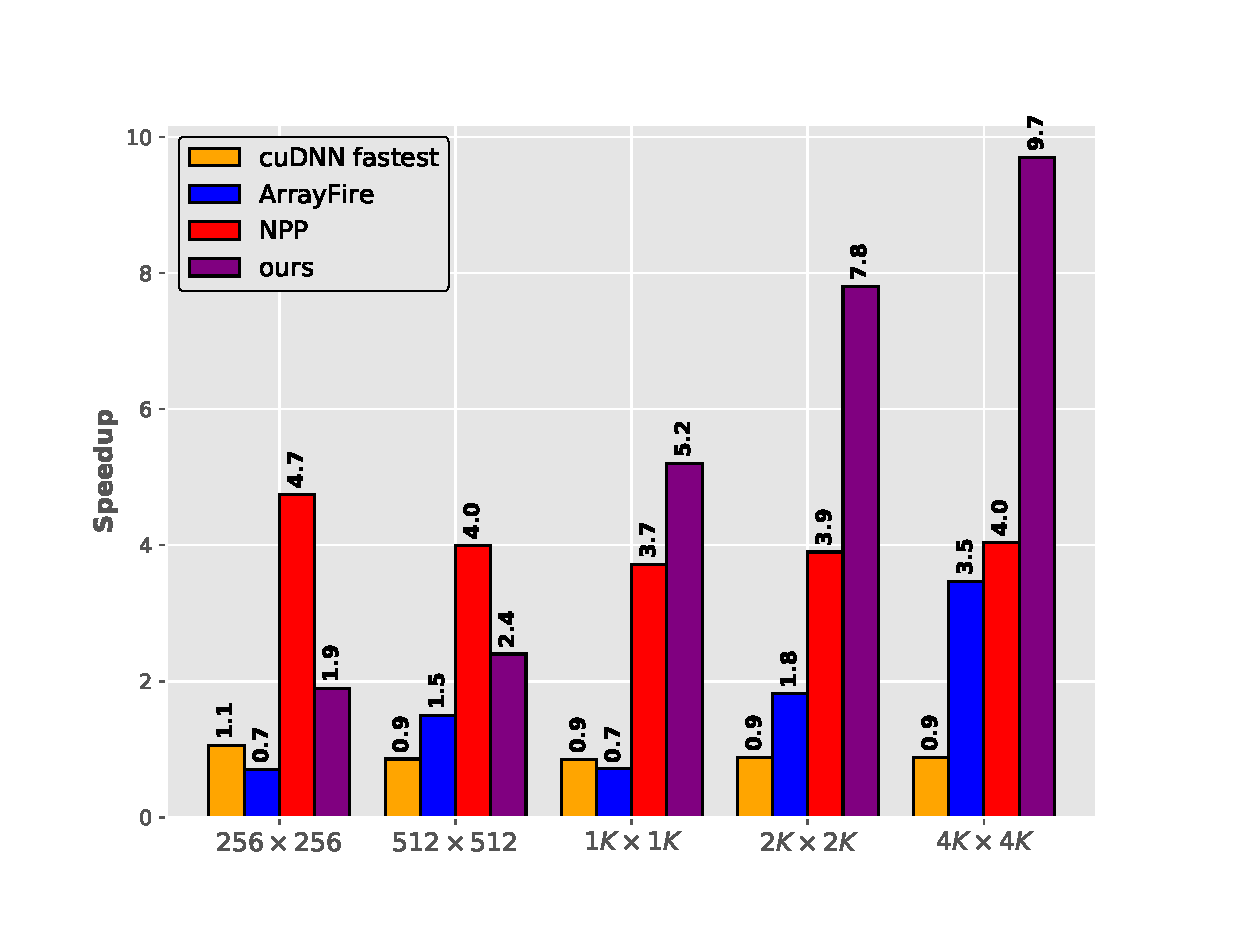
\includegraphics[width=0.85\columnwidth,height=4.5cm]{./figure/2d_conv_f3.eps}
	\label{fig:2druntimef3c12080}}
\hspace{0em}
\subfloat[][Speedups when using a $3 \times 3$ filter]{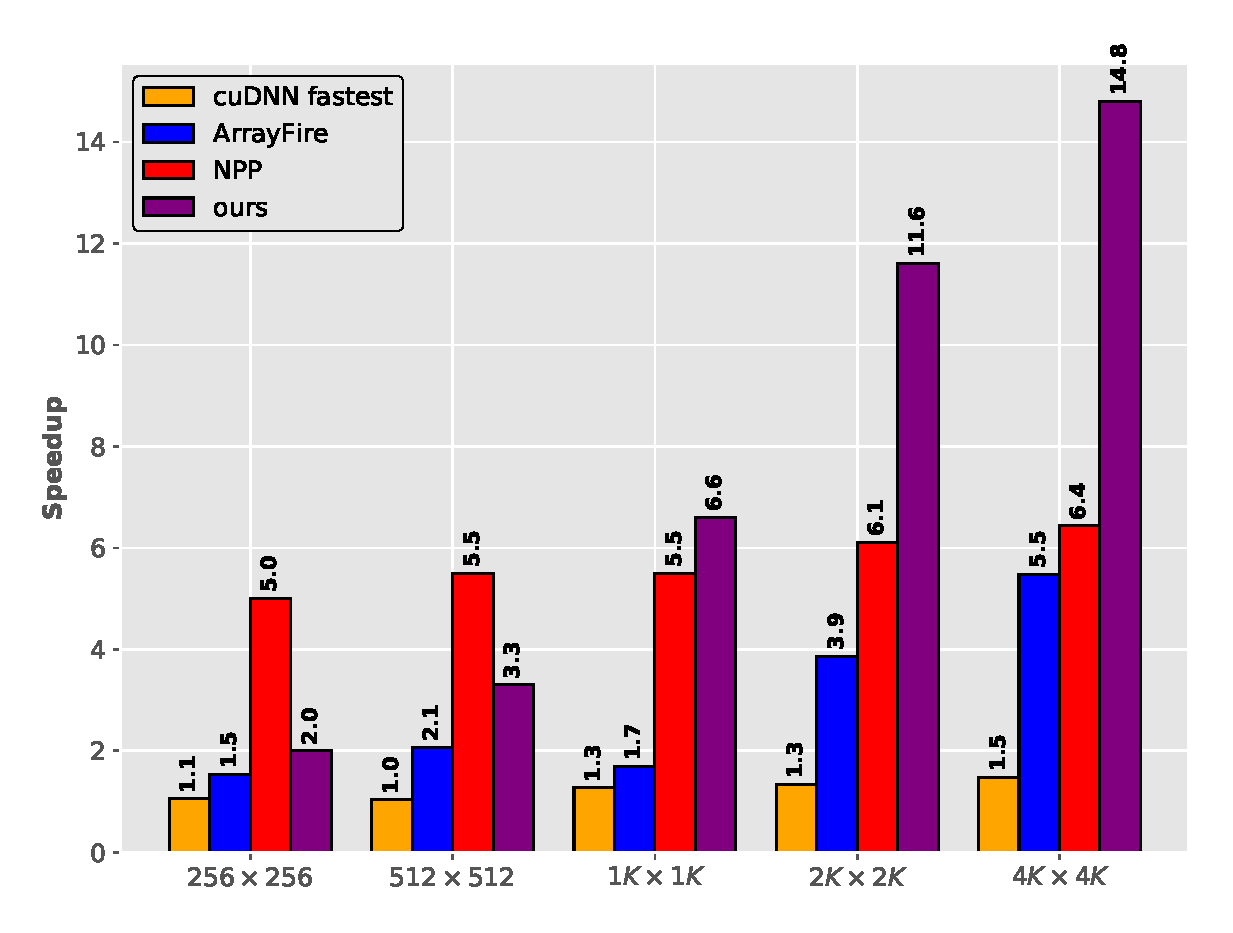
\includegraphics[width=0.85\columnwidth,height=4.5cm]{./figure/2d_conv_f5.eps}
	\label{fig:2druntimef5c12080}}
	
\caption{Speedups of 2D convolutions of four implementations over GEMM-im2col when using a $3 \times 3$ (a) and a $5 \times 5$ filter (b).}
\label{fig:2druntime}
\vspace{-3mm}
\end{figure*}


\subsubsection{Setup}
In this experiment, we compare our approach against the single-channel 2D convolution implementation from cuDNN, im2col, ArrayFire, and
NPP. As cuDNN provides multiple implementations, we empirically choose the fastest version, denoted as cuDNN-fastest, for evaluation. We
apply each method to images with sizes ranging from $256 \times 256$ to $4K \times 4K$. We set the batch size, channel, height, and width
of the input to be 1.


\subsubsection{Overall results}
 Figure
\ref{fig:2druntime} reports the speedups of cuDNN, ArrayFire, NPP and our approach over GEMM-im2col. While cuDNN has been heavily optimized
for NVIDIA GPUs, it does not show a notable performance advantage. When using a $3 \times 3$ filter, our approach gives the best overall
speedup of 6.5x (up to 9.7x for the largest input), which translates to an improvement of  more than 30\% over the second-best method, NPP.
We note that our approach is based on the standard 2D direct convolution by applying the column and row reuse algorithms. Therefore, the
performance gain is mainly attributed to the reduction of the number of memory transactions. When using a $5 \times 5$ filter, our approach
achieves a better overall speedup of $7.7\times$. A $5 \times 5$ filter has four overlapped columns and rows (instead of just one
overlapped column and row on width and height dimensions when using a $3 \times 3$ filter). The larger number of overlapped data thus give
more room for performance optimization when using our column and row reuse algorithms. Our approach achieves the best overall performance
and demonstrates significant performance advantages when processing large input.

\subsubsection{Further analysis}
\begin{figure}[t!]
\centering

\subfloat[][Memory throughput]{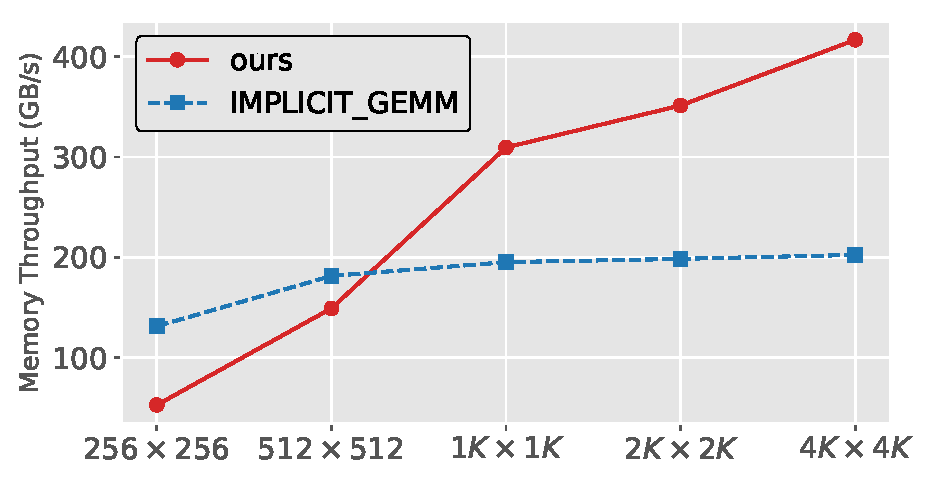
\includegraphics[width=0.85\columnwidth]{./figure/2dmemthroughput.eps}
	\label{fig:2dmemthr}}

\subfloat[][Maximum memory bandwidth]{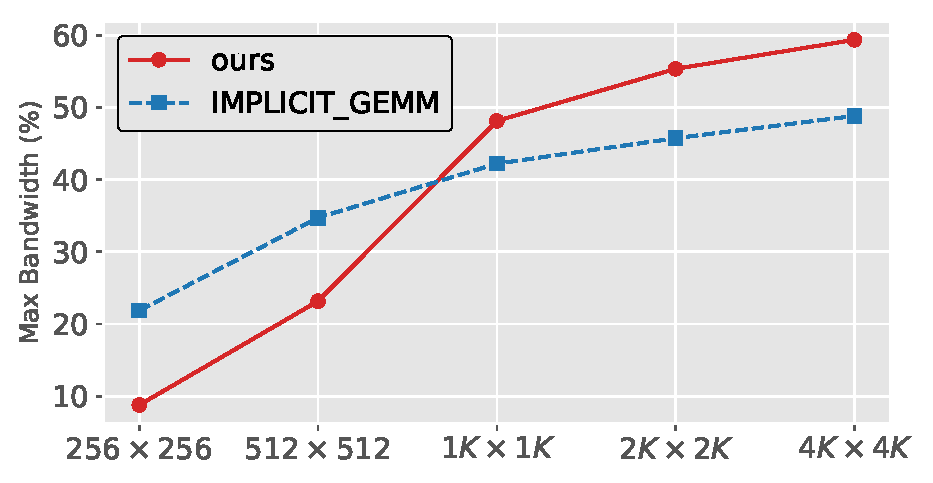
\includegraphics[width=0.85\columnwidth]{./figure/2dmembandwidth.eps}
	\label{fig:2dmaxband}}
	
\caption{Memory throughput (a) and maximum memory bandwidth (b) of NPP and our implementation for the filter of size $3 \times 3$.}
\label{fig:2dmemanaly}
\vspace{-5mm}
\end{figure}

On the test cases of small input sizes (i.e., $256 \times 256$ and $512 \times 512$), NPP gives the best performance. To understand the
performance gap on small input sizes, we use \emph{nvidia compute} to collect memory profiles, including memory throughput and max
bandwidth, of our implementation and NPP when using a $3 \times 3$ filter to perform convolution. The profiling results are shown in Figure
\ref{fig:2dmemanaly}.  We see that as the input size increases, the memory throughput and the maximum bandwidth also grow. This is expected
as the larger the input image, the larger number the memory transactions is likely to be when performing convolution.  We also observe that
our approach leads to higher memory throughput and the maximum bandwidth used when the input image size is greater or equal than $1K \times
1K$. This finding matches the results presented in Figure \ref{fig:2druntime}, where our approach gives the best performance when
processing an image whose size is $1K \times 1K$ or larger. This result also suggests that memory performance has a strong correlation with
the performance of 2D convolutions.


The reason why our approach gives lower memory throughput and achieves lower maximum bandwidth on small input sizes over NPP is explained
as follows. For single-channel 2D convolution, only one filter is used to convolve with one single-channel input feature map, which
requires much less computation compared to, e.g., the depth-wise or multi-channel 2D convolutions. Therefore, memory performance has a huge
impact on the performance of 2D convolutions. Our row reuse algorithm performs better when a thread operates on more rows of output.
However, the more rows a thread compute on, the fewer warps and thread blocks we can generate. Without enough warps issuing memory
requests, the memory throughput and maximum bandwidth will reduce significantly, which leads to slower performance over NPP. As the input
size increases, we can allocate more thread blocks and more warps per thread block. With enough memory requests and reduction on redundant
memory transactions, we can increase the memory throughput and max bandwidth to improve the performance of 2D convolution.



%Our approach achieves the best speedups in six out of ten test cases. NPP achieves the best results on small image sizes, whereas our
%implementation demonstrates the best results on large image sizes. We use \emph{nvidia compute} to collect memory profiles, including
%memory throughput and max bandwidth, of our implementation and NPP when convolving with a $3 \times 3$ filter. The results are shown in
%Figure \ref{fig:2dmemanaly}.
%
%We can see that as the input size increases, memory throughput and max bandwidth of our implementation exceeds that of NPP, the turning point ($1K \times 1K$ in Figure \ref{fig:2dmemanaly}) is the same as that of speedups in Figure \ref{fig:2druntimef3c12080}, which means that memory performance has a strong relationship with the performance of 2D convolutions. Next, we give a detailed analysis of why the memory throughput and max bandwidth of our implementation is low for small input sizes.
%
%When performing 2D convolutions, only one filter is used to convolve with one single-channel input feature map, which requires much less computation than depth-wise convolutions. Therefore, the memory performance has a huge impact on the performance of 2D convolutions. The proposed row reuse algorithm performs better when a thread calculates more rows of output. However, the more rows each thread calculates, the less warps and thread blocks we can generate. Without enough warps issuing memory requests, the memory throughput and max bandwidth can reduce a lot, which can slow down our implementations. As the input size increases, we can allocate more thread blocks and more warps per thread block. With enough memory requests and reduction on redundant memory transactions, we can increase the memory throughput and max bandwidth, and thus improve the performance of our implementation.
%
%The average speedup of our implementation for $5 \times 5$ filter is $7.7\times$, which is better than the speedup of $5.4\times$ for $3 \times 3$ filter. The key reason for the improvement is that, for $3 \times 3$ filter, there is only one overlapped column and row on width and height dimensions. While for $5 \times 5$ filter, there are four overlapped columns and rows, therefore column and row reuse algorithms can be used more efficiently compared with  that for the $3 \times 3$ filter.





\subsubsection{Summary} Overall, our optimization algorithms can greatly reduce the number of memory transactions and improve the performance of 2D
convolutions. Compared with state-of-the-art image processing libraries, NPP, our approach achieves average speedups of 1.3$\times$ and
1.28$\times$ when using a $3 \times 3$ and $5 \times 5$ filters, respectively.

\subsection{Depth-wise Convolution}
\label{sec:depconvexp}

\begin{table}[]
\caption{Layer configurations of depth-wise  convolutions$^{\dag}$.}
\label{tab:3dconvconfigs}
\centering
\rowcolors{2}{}{Gray}
\begin{threeparttable}
\begin{tabular}{lrrrrr}
\toprule
& \textbf{$I_N$} & \textbf{$I_C$} & \textbf{$I_H \times I_W$ }&  \textbf{$F_H \times F_W$} \\
\midrule
\textbf{CONV1} & 512  & 32    & 112*112 & $3 \times 3$, $5 \times 5$  \\
\textbf{CONV2} & 512  & 96    & 112*112  &$3 \times 3$, $5 \times 5$   \\
\textbf{CONV3} & 512  & 144   & 56*56  &$3 \times 3$, $5 \times 5$    \\
\textbf{CONV4} & 512  & 160    & 56*56  &$3 \times 3$, $5 \times 5$    \\
\textbf{CONV5} & 512  & 192   & 28*28  &$3 \times 3$, $5 \times 5$    \\
\textbf{CONV6} & 512  & 240   & 28*28  &$3 \times 3$, $5 \times 5$    \\
\textbf{CONV7} & 512  & 256   & 28*28  &$3 \times 3$, $5 \times 5$    \\
\textbf{CONV8} & 512  & 384   & 14*14  &$3 \times 3$, $5 \times 5$    \\
\textbf{CONV9} & 512  & 480   & 14*14  &$3 \times 3$, $5 \times 5$    \\
\textbf{CONV10} & 512  & 672  & 14*14 &$3 \times 3$, $5 \times 5$     \\
\textbf{CONV11} & 512  &672  & 7*7 & $3 \times 3$, $5 \times 5$      \\
\textbf{CONV12} & 512  &960  & 7*7 & $3 \times 3$, $5 \times 5$      \\
\textbf{CONV13} & 512  &1152  & 7*7 & $3 \times 3$, $5 \times 5$      \\
\bottomrule
\end{tabular}
\footnotesize
\begin{tablenotes}
\item[\dag] We use $I$, $F$, and $O$ to represent the input, the filter, and the output respectively, $N$, $C$, $H$, and $W$
to denote the batch size, the channel, the height, and the width, respectively.
\end{tablenotes}
\end{threeparttable}
\vspace{-5mm}
\end{table}

\begin{figure*}
\centering
	
\subfloat[][$3\times 3$ filter]{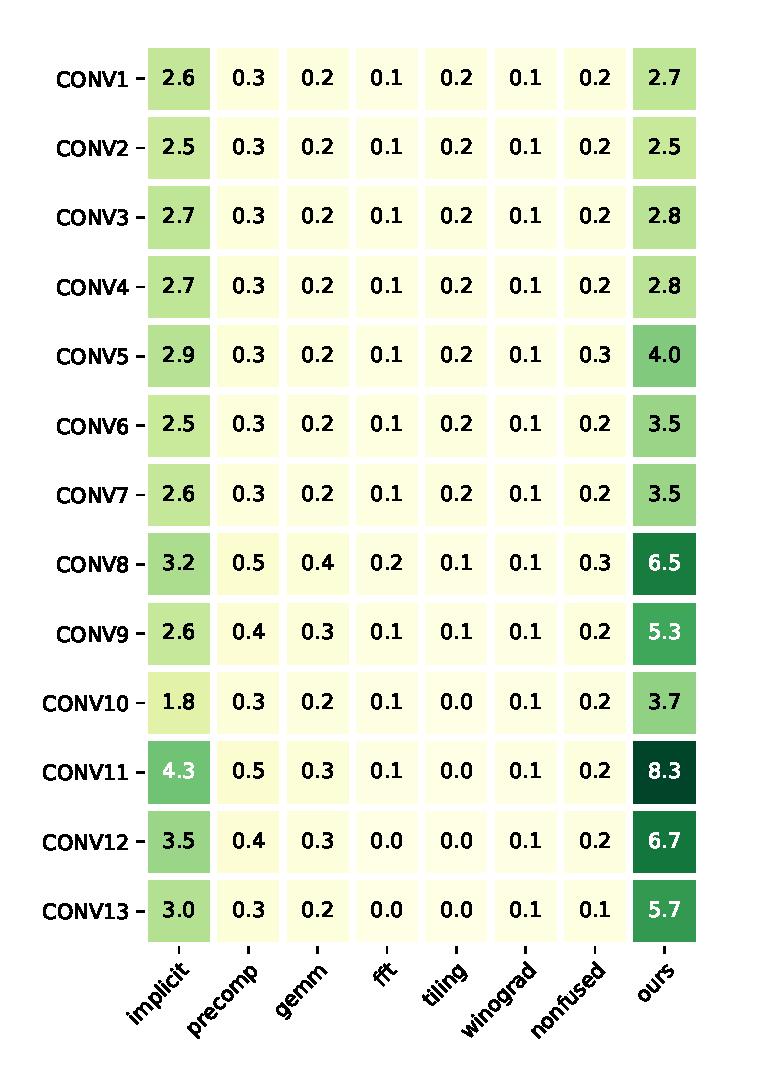
\includegraphics[width=0.9\columnwidth]{./figure/depthwise_f3.eps}
	\label{fig:f33druntime2080}}
\subfloat[][$5\times 5$ filter]{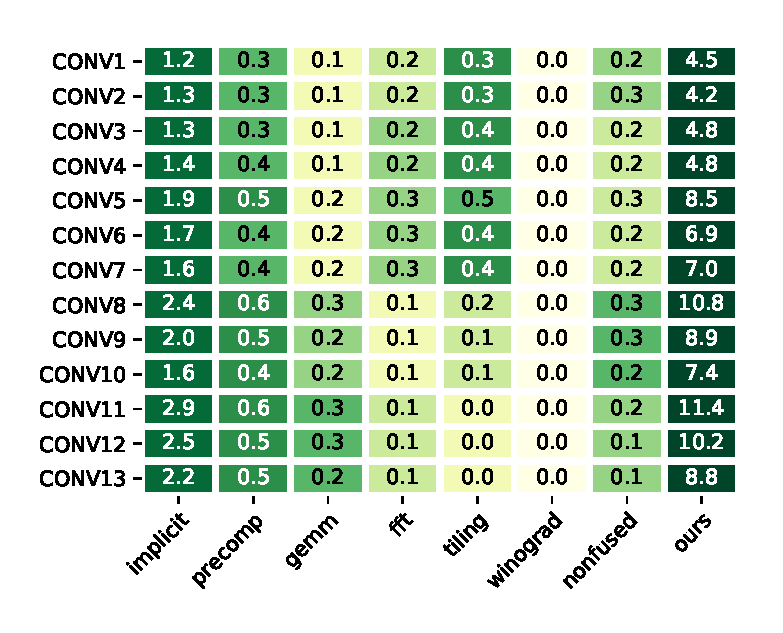
\includegraphics[width=0.9\columnwidth]{./figure/depthwise_f5.eps}
	\label{fig:f53druntime2080}}

\vspace{-2mm} \caption{Speedups of our approach and cuDNN over the baseline implementation of the depth-wise convolution when using a
$3\times 3$ (a) and a $5\times 5$ filter (b).} \label{fig:3druntime}
\vspace{-2mm}
\end{figure*}


\subsubsection{Setup} In this experiment, we compare our approach against the depth-wise
convolution implementations of cuDNN. Specifically, we compare to seven algorithms in cuDNN, including IMPLICIT\_GEMM (implicit),
IMPLICIT\_PRECOMP\_GEMM (precomp), GEMM (gemm), FFT (fft), FFT\_TILING (tiling), WINOGRAD (winograd) and WINOGRAD\_NONFUSED (nonfused). As
Winograd is not applicable  to a $5 \times 5$ filter, we do not report performance of Winograd when using a $5 \times 5$ filter. As a
baseline, we implement a simple depth-wise convolution. We use the convolutional layer configurations that apply depth-wise convolution
from three popular embedded models, MobileNetv2, ShuffleNetv2 and EfficientNet. We report the performance when the input and output batch
sizes are set to 512, but we observe similar performance when using a different batch size. Table \ref{tab:3dconvconfigs} gives the layer
configurations used in this experiment.


%In the depth-wise convolution, one input element only needs to be convolved with
%one filter, while in the multi-channel 2D convolution, one input element needs to be convolved with all filters. Therefore, depth-wise
%convolutions require much less computation than multi-channel 2D convolutions, which makes depth-wise convolutions more sensitive to memory
%performance.


%Nowadays, depth-wise convolutions have been widely used in embedded CNNs, including MobileNetv2 \cite{Sandler_2018_CVPR}, EfficientNet
%\cite{tan2019efficientnet} and ShuffleNetv2 \cite{Ma_2018_ECCV}. In this section, we present the performance comparison of the depth-wise
%convolution between cuDNN and our implementation. We implement a simple depth-wise convolution and report speedups of cuDNN and our
%implementation over the simple depth-wise convolution. We evaluate 7 algorithms in cuDNN, including IMPLICIT\_GEMM (implicit),
%IMPLICIT\_PRECOMP\_GEMM (precomp), GEMM (gemm), FFT (fft), FFT\_TILING (tiling), WINOGRAD (winograd) and WINOGRAD\_NONFUSED (nonfused).
%Winograd can not be applied on a $5 \times 5$ filter, thus we set speedups for this algorithm to 0.

%We collect configurations of the convolutional layers using depth-wise convolution from three popular mobile embedded models,
%namely, MobileNetv2, ShuffleNetv2 and EfficientNet.
%Then, we set the number of the batch size to 512 ($I_N=O_N=512$). Other batch sizes demonstrate a similar performance because all tested implementations have a linear scale as the batch size. The exact configuration is presented in Table \ref{tab:3dconvconfigs}.

\subsubsection{Overall results.}
Figure \ref{fig:3druntime} shows that our approach gives the best speedup. Our approach delivers an average speedup of $4.5\times$ and
$7.6\times$ for the $3 \times 3$ and $5 \times 5$ filters, respectively. The implicit algorithm is the fastest algorithm in cuDNN in all
test cases. It achieves an average speedup of $2.8\times$ and $1.8\times$ for the $3 \times 3$ and $5 \times 5$ filters, respectively.
Other algorithms of cuDNN except implicit algorithm perform poorly in all test cases. Since that cuDNN is a closed source, we cannot
investigate the source code for further analysis. We hypothesize that FFT- and Winograd- based algorithms focus on reduction of computation
and trades memory performance for speed. Precomp and gemm algorithms need extra memory operations to compute output elements. Moreover,
depth-wise convolution is more sensitive to memory performance than multi-channel 2D convolution. Consequently, these algorithms are not suitable for
depth-wise convolutions. Over all, our approach improves \emph{implicit} by $1.5\times$ (up o $2\times$) and $2\times$ (up to $4.5\times$)
when using a $3 \times 3$ and $5 \times 5$ filter respectively.

%
%The algorithms of cuDNN except implicit algorithm perform poorly in all test cases and the speedups of these algorithms all below 1.
%Considering that cuDNN is a closed source, we can only guess that FFT- and Winograd- based algorithms focus on reduction of computation and
%trades memory performance for speed. Precomp and gemm algorithms need extra memory operations to compute output elements. Moreover,
%depth-wise convolution is more sensitive to memory performance than multi-channel 2D convolution. Consequently, these algorithms perform
%poorly on depth-wise convolutions.

\begin{figure}[t!]
\centering

\subfloat[][Memory throughput]{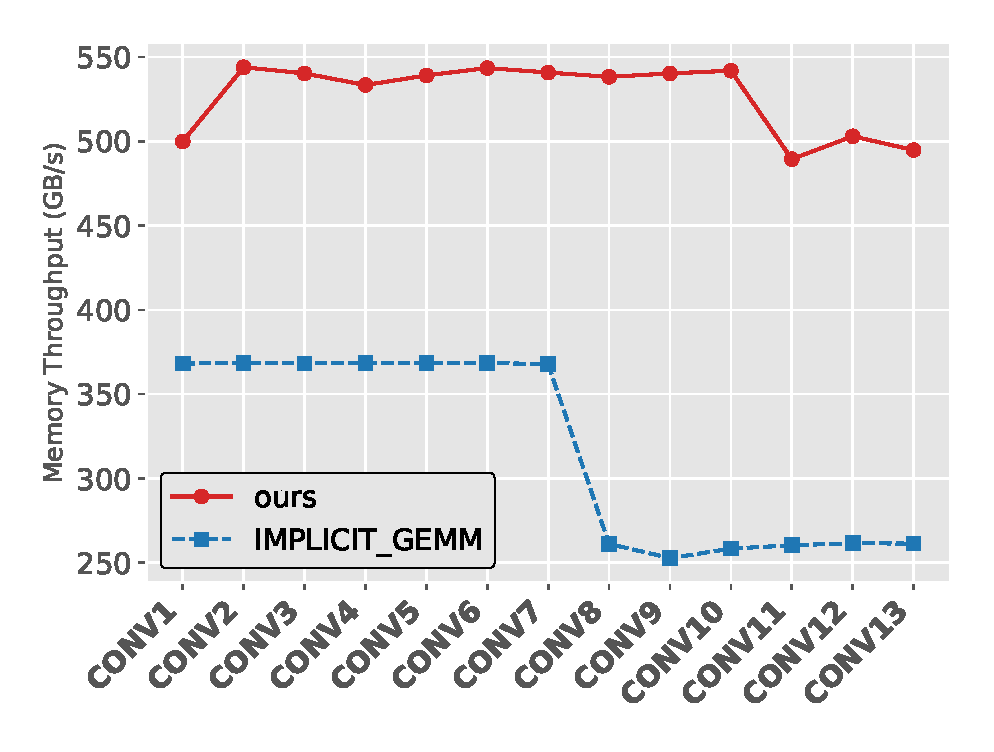
\includegraphics[width=0.85\columnwidth]{./figure/depwisememthroughput.eps}
	\label{fig:depwisememthr}} \hspace{0em}


\subfloat[][Maximum bandwidth]{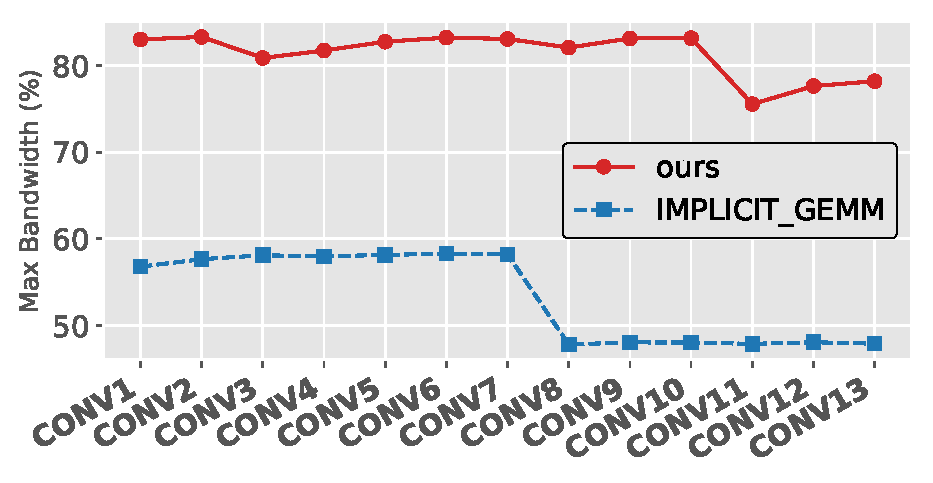
\includegraphics [width=0.85\columnwidth]{./figure/depwisemembandwidth.eps}
	\label{fig:depwisemaxband}}
	
\caption{Memory throughput (a) and maximum bandwidth (b) of cuDNN implicit algorithm and our implementation for the filter of size $3 \times 3$.}
\label{fig:depwisememanaly}
\vspace{-2mm}
\end{figure}

\subsubsection{Further analysis}
Figure \ref{fig:depwisememanaly} reports the measured memory throughput and maximum memory bandwidth for our approach and the fast cuDNN
\emph{implicit} algorithm when using a $3 \times 3$ filter. Our approach achieves $1.5 \times$ higher memory throughput and maximum
bandwidth compared with the \emph{implicit} algorithm. This suggests that our reuse algorithms can improve memory performance significantly, which
thus lead to better computational performance.


\subsubsection{Summary}
Our approach can significantly improve the memory throughput and maximum bandwidth, which leads to faster computation time when performing
depth-wise convolutions.  Compared to the fastest available algorithms in cuDNN, which is the state-of-the-art convolution library, our
approach achieves an average speedup of $1.5\times$ and $4\times$ when using a $3 \times 3$ and $5 \times 5$ filter, respectively.


\subsection{Multi-channel 2D Convolution}
\label{multicconvexp}

\begin{table}[]
\caption{Layer configurations used for multi-channel 2D convolutions$^{\dag}$.}
\label{tab:3dconvconfigs}
\rowcolors{2}{}{Gray}
\begin{threeparttable}
\begin{tabular}{lrrrrr}
\toprule
& \textbf{$I_N$} & \textbf{$I_C=F_C$} & \textbf{$I_H \times I_W$} & \textbf{$F_N$} & \textbf{$F_H \times F_W$} \\
\midrule
\textbf{CONV1} & 128  & 1,3       & $28\times 28$     & 128  & $3\times 3$       \\
\textbf{CONV2} & 128  & 1,3       & $56\times 56$     & 64   & $3\times 3$       \\
\textbf{CONV3} & 128  & 1,3       & $12\times 12$     & 64   & $5\times 5$       \\
\textbf{CONV4} & 128  & 1,3       & $14\times 14$     & 16   & $5 \times 5$       \\
\textbf{CONV5} & 128  & 1,3       & $24\times 24$    & 256  & $5 \times 5$       \\
\textbf{CONV6} & 128  & 1,3       & $24\times 24$     & 64   & $5\times 5$       \\
\textbf{CONV7} & 128  & 1,3       & $28\times 28$     & 16   & $5\times 5$       \\
\textbf{CONV8} & 128  & 1,3       & $28\times 28$     & 512   & $3\times 3$       \\
\textbf{CONV9} & 128  & 1,3       & $56\times 56$     & 256  & $3\times 3$       \\
\textbf{CONV10} & 128  & 1,3       & $112\times 112$     & 128   & $3\times 3$       \\
\textbf{CONV11} &128  & 1,3       & $224\times 224$     & 64   & $3\times 3$      \\
\bottomrule
\end{tabular}
\begin{tablenotes}
\item[\dag] We use $I$, $F$, and $O$ to represent the input, the filter, and the output respectively, $N$, $C$, $H$, and $W$
to denote the batch size, the channel, the height, and the width, respectively.
\end{tablenotes}
\end{threeparttable}
\end{table}

\begin{figure*}
\centering
	
\subfloat{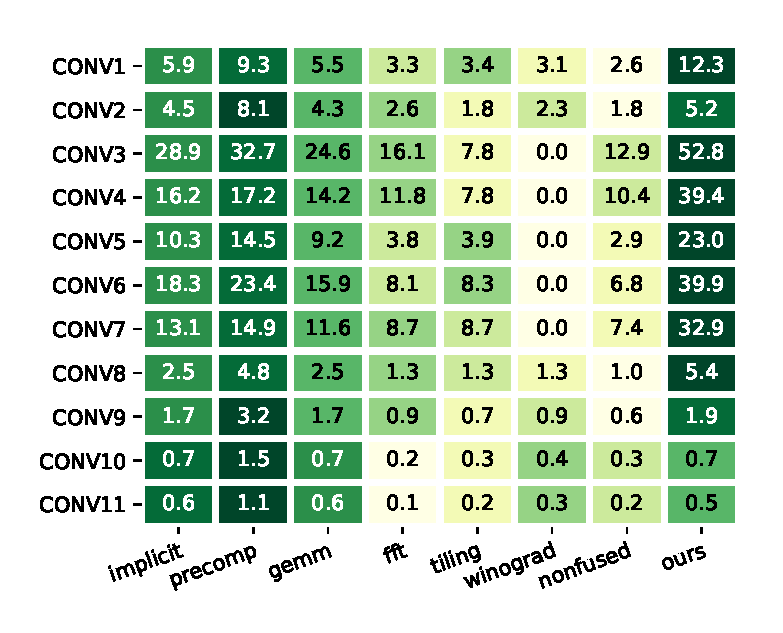
\includegraphics[width=0.9\columnwidth,height=5.5cm]{./figure/multic2d_c1.eps}
	\label{fig:multic1runtime2080}}
\subfloat{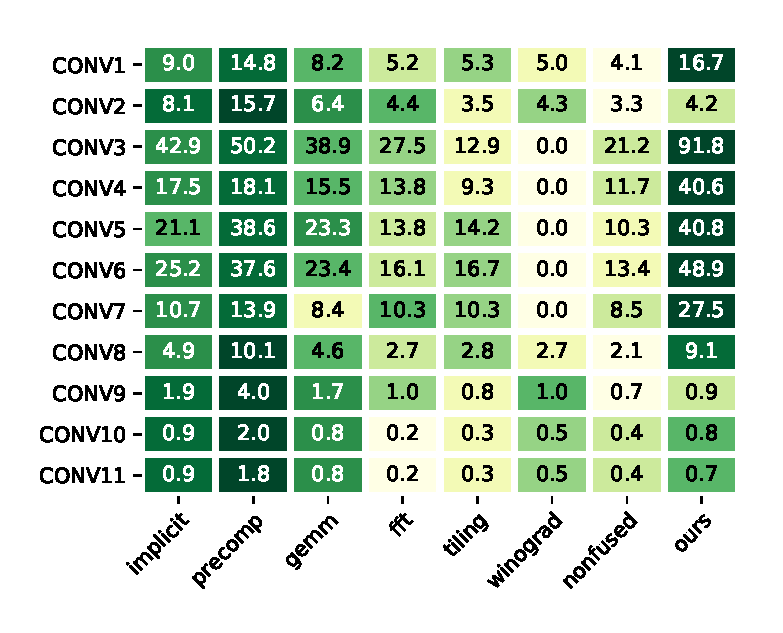
\includegraphics[width=0.9\columnwidth,height=5.5cm]{./figure/multic2d_c3.eps}
	\label{fig:multic3runtime2080}}
\vspace{-2mm}
\caption{Speedups of our approach and cuDNN over GEMM-im2col for one (left) and three (right) input channels.} \label{fig:multi2druntime}
\vspace{-2mm}
\end{figure*}


\subsubsection{Setup} In this experiment, we compare our approach against the multi-channel 2D convolution implementations in cuDNN and use GEMM-im2col as the baseline. Since our work focuses on optimizing memory transactions of convolutions but not operations on input channels, we apply our approach to convolutions with one and three input channels, which are typically used in the first few layers of a CNN. We use the layer configurations four popular CNN models,
namely, AlexNet \cite{Krizhevsky2012ImageNet}, VGG \cite{SimonyanZ14a}, ResNet \cite{HeZRS16} and GoogleLeNet \cite{SzegedyLJSRAEVR15}. We
use $3 \times 3$ and $5 \times 5$ filters with a batch size of 128. Table \ref{tab:3dconvconfigs} lists the layer configurations used in
this experiment.

\subsubsection{Results} Figure \ref{fig:multi2druntime} shows that our
implementation achieves an average speedup of 19.5$\times$ and 25.6$\times$ over GEMM-im2col for one and three input channels,
respectively. This translates to an improvement of 1.23$\times$ and 1.13$\times$ over the fastest algorithm in cuDNN, for one and three
input channels, respectively. Since our approach does not optimize for input channels, it does not give performance improvement for layer
configurations that have a large number of channels (e.g., CONV10 and CONV11). This can be improved by \FIXME{Explain how you can improve
this.}. Nonetheless, our approach significantly boosts the performance for convolution layers with a small number of channels (which is the
typical case for many CNNs).

\section{Related Work}
Numerous efforts have been dedicated to optimizing convolution operations. As previously mentioned, GEMM-, FFT- and
Winograd-based convolutions are broadly adopted convolution algorithms.

GEMM-based convolution is the first attempt to optimize convolution. Chellapilla et al. \cite{Chellapilla2006High} developed an unrolling
convolution algorithm  called the im2col convolution algorithm. They lowered the convolutions into a matrix multiplication, which is
highly optimized on GPUs. Despite some duplicate input elements involved in the computation, the performance gain of this algorithm is impressive.

FFT- and Winograd-based convolutions can reduce computational complexity and improve convolution performance. Mathieu et al.
\cite{mathieu2013fast} proposed an FFT-based convolution to compute convolutions as pointwise products in the Fourier domain and reuse the
transformed input data, which significantly reduces the complexity of the convolution. However, FFT-based convolution is more suitable for large filters than
for small ones. Because padding the filters to the same size as the input data is necessary, and  the latter (e.g., $3 \times 3$ filters) needs
more memory than the former. Lavin et al. \cite{lavin2016fast} used Winograd's minimal filtering algorithm to
accelerate the convolution on GPU. This algorithm can reduce the arithmetic complexity of convolution by up to four times compared with
direct convolution. However, Winograd's algorithm is only suitable for small filters due to its numerical instability.
Zhen et al. \cite{Zhen2018Optimizing} extended Winograd's algorithm to support any filter size. However, the traditional and extended Winograd-based
algorithms need to transform the input and filter before performing matrix multiplication, and both require more operations than the FFT algorithm.

Transforming the input and filter before performing matrix multiplication incurs a large memory overhead, which can outweigh the
performance gains obtained through lowering the computational complexity. Therefore, recent studies have looked into minimizing the memory
overhead of the transformation phases. Cho et al. \cite{cho2017mec} reduced the memory overhead of GEMM-based convolutions using a compact
lowering scheme to reduce the redundancy in the lowered matrix and then performed multiple small matrix multiplications in parallel.
However, this algorithm still needs to transform the input and filter tensors into lowered matrixes to compute the convolution. Iandola et
al. \cite{Iandola2014Communication} reduced memory communication of 2D convolutions on GPU. They also prefetched the image regions to the
registers. While their method uses fewer threads, each thread operates on a larger number of data items. As a result, their method does not
reduce the number of global memory transactions. Unlike \cite{Iandola2014Communication}, our approach promotes register use and can
significantly reduce the number of memory accesses.

\section{Conclusion}
We have presented a novel approach to optimize the memory access for convolution computation on GPUs. Our approach improves the data
locality for convolutional operations performed on the row and column directions to reduce the memory access. Our techniques utilize the
common GPU shuffle operations supported by mainstream GPU programming models, including CUDA and OpenCL, and do not require hardware
modifications. We evaluate our approach by applying it to 2D, depth-wise and multi-channel 2D convolutions and evaluate it on an NVIDIA RTX
2080Ti GPU platform. For the 2D convolution, our approach doubles the performance of the state-of-the-art image processing libraries. For
the depth-wise convolution, our techniques deliver up to $4 \times$ speedups over the fastest algorithm of cuDNN. For the multi-channel 2D
convolution, proposed reuse algorithms achieve an average speedup of $1.23\times$ over the fastest algorithm of cuDNN.


%\begin{acks}                            %% acks environment is optional
%                                        %% contents suppressed with 'anonymous'
%  %% Commands \grantsponsor{<sponsorID>}{<name>}{<url>} and
%  %% \grantnum[<url>]{<sponsorID>}{<number>} should be used to
%  %% acknowledge financial support and will be used by metadata
%  %% extraction tools.
%  This material is based upon work supported by the
%  \grantsponsor{GS100000001}{National Science
%    Foundation}{http://dx.doi.org/10.13039/100000001} under Grant
%  No.~\grantnum{GS100000001}{nnnnnnn} and Grant
%  No.~\grantnum{GS100000001}{mmmmmmm}.  Any opinions, findings, and
%  conclusions or recommendations expressed in this material are those
%  of the author and do not necessarily reflect the views of the
%  National Science Foundation.
%\end{acks}


\section*{Acknowledgments}
This work was supported in part by the National Key Research and Development Program of China under Grant agreement 2017YFB0202901, the
Key-Area Research and Development Program of Guangdong Province under Grant agreement 2019B010136001, the National Natural Science
Foundation of China (NSFC) under Grant agreement 61672186 and 61872294, and the Shenzhen Technology Research and Development Fund under
Grant agreement JCYJ20190806143418198. Professor Zhang is the corresponding author.

%% Bibliography
%\bibliographystyle{IEEEtran}
%\bibliography{IEEEabrv,ref}
%\begin{IEEEbiography}[{
\includegraphics[width=1in,height=1.25in,clip,keepaspectratio]{./figure/GangzhaoLu.eps}}]{Gangzhao Lu}
% received the B.S. degree in computer science and engineering from Harbin Institute of Technology, China, in 2014. He is currently working toward the Ph.D. degree in the School of Cyberspace Science, Harbin Institute of Technology. His research interests include performance modeling, parallel optimization, auto-tuning.
%\end{IEEEbiography}
%\begin{IEEEbiography}[{
\includegraphics[width=1in,height=1.25in,clip,keepaspectratio]{./figure/WeizheZhang.eps}}]{Weizhe Zhang} (Senior Member, IEEE) received B.Eng, M.Eng and Ph.D. degree of Engineering in computer science and technology in 1999, 2001 and 2006 respectively from Harbin Institute of Technology.
%
%He is currently a professor in the School of Computer Science and Technology at Harbin Institute of Technology, China, and director in the Cyberspace Security Research Center, Peng Cheng Laboratory, Shenzhen, China. His research interests are primarily in parallel computing, distributed computing, cloud and grid computing, and computer network. He has published more than 100 academic papers in journals, books, and conference proceedings.
%\end{IEEEbiography}
%\begin{IEEEbiography}[{
\includegraphics[width=1in,height=1.25in,clip,keepaspectratio]{./figure/ZhengWang.eps}}]{Zheng Wang} is
%an associate professor with the University of Leeds. His research focuses on parallel computing, compilation and systems security.
%\end{IEEEbiography}
\end{document}
